%%
%% Copyright 2019-2021 Elsevier Ltd
%%
%% This file is part of the 'CAS Bundle'.
%% --------------------------------------
%%
%% It may be distributed under the conditions of the LaTeX Project Public
%% License, either version 1.2 of this license or (at your option) any
%% later version.  The latest version of this license is in
%%    http://www.latex-project.org/lppl.txt
%% and version 1.2 or later is part of all distributions of LaTeX
%% version 1999/12/01 or later.
%%
%% The list of all files belonging to the 'CAS Bundle' is
%% given in the file `manifest.txt'.
%%
%% Template article for cas-sc documentclass for
%% single column output.

\documentclass[a4paper,fleqn]{cas-sc}

% If the frontmatter runs over more than one page
% use the longmktitle option.

%\documentclass[a4paper,fleqn,longmktitle]{cas-sc}

\usepackage[numbers]{natbib}
%\usepackage[authoryear]{natbib}
%\usepackage[authoryear,longnamesfirst]{natbib}
%%%Author macros
\def\tsc#1{\csdef{#1}{\textsc{\lowercase{#1}}\xspace}}
\tsc{WGM}
\tsc{QE}
%%%

% Uncomment and use as if needed
%\newtheorem{theorem}{Theorem}
%\newtheorem{lemma}[theorem]{Lemma}
%\newdefinition{rmk}{Remark}
%\newproof{pf}{Proof}
%\newproof{pot}{Proof of Theorem \ref{thm}}

\begin{document}
\let\WriteBookmarks\relax
\def\floatpagepagefraction{1}
\def\textpagefraction{.001}

% Short title
\shorttitle{Impact of Iron Defect Variability on Silicon Solar Cell Performance}

% Short author
\shortauthors{O.Olikh, O.Zavhorodnii}

% Main title of the paper
\title [mode = title]{Modeling the Impact of Iron Defect Variability on Silicon Solar Cell Performance Across Different Scenarios}

% Title footnote mark
% eg: \tnotemark[1]
%\tnotemark[<tnote number>]

% Title footnote 1.
% eg: \tnotetext[1]{Title footnote text}
%\tnotetext[<tnote number>]{<tnote text>}

% First author
%
% Options: Use if required
% eg: \author[1,3]{Author Name}[type=editor,
%       style=chinese,
%       auid=000,
%       bioid=1,
%       prefix=Sir,
%       orcid=0000-0000-0000-0000,
%       facebook=<facebook id>,
%       twitter=<twitter id>,
%       linkedin=<linkedin id>,
%       gplus=<gplus id>]

%\author[1,3]{Oleg Olikh}[type=Co-ordinator,
%       style=chinese,
%       auid=000,
%       bioid=1,
%       prefix=Dr.,
%       orcid=0000-0003-0633-5429,
%%       facebook=<facebook id>,
%%       twitter=<twitter id>,
%%       linkedin=<linkedin id>,
%       gplus=<gplus id>]
\author{Oleg Olikh}[
%       type=Co-ordinator,
%       style=chinese,
%       auid=000,
%       bioid=1,
%       prefix=Dr.,
       orcid=0000-0003-0633-5429
       % ,
%       facebook=<facebook id>,
%       twitter=<twitter id>,
%       linkedin=<linkedin id>,
%       gplus=<gplus id>
       ]

% Corresponding author indication
\cormark[1]

% Footnote of the first author
%\fnmark[1]

% Email id of the first author
\ead{olegolikh@knu.ua}

% URL of the first author
%\ead[url]{https://gen.phys.univ.kiev.ua/280-olikh/}

% Credit authorship
% eg: \credit{Conceptualization of this study, Methodology, Software}
%\credit{<Credit authorship details>}

% Address/affiliation
\affiliation{organization={Taras Shevchenko National University of Kyiv},
            addressline={64/13, Volodymyrska Street},
            city={Kyiv},
%          citysep={}, % Uncomment if no comma needed between city and postcode
            postcode={01601},
 %           state={},
            country={Ukraine}}

%\affiliation[<aff no>]{organization={Taras Shevchenko National University of Kyiv, Faculty of Physics},
%            addressline={ave Glushkov 2},
%            city={Kyiv},
%%          citysep={}, % Uncomment if no comma needed between city and postcode
%            postcode={03022},
%            state={},
%            country={Ukraine}}

%\author[1,3]{Zavhorodnii Oleksii}[type=editor,
%       style=chinese,
%       auid=000,
%       bioid=1,
%%       prefix=Mr,
%       orcid=0000-0001-8080-7661,
%%       facebook=<facebook id>,
%%       twitter=<twitter id>,
%%       linkedin=<linkedin id>,
%       gplus=<gplus id>]

\author{Oleksii Zavhorodnii}[
       orcid=0000-0001-8080-7661]

% Footnote of the second author
%\fnmark[2]

% Email id of the second author
\ead{nevermor464@gmail.com}

% URL of the second author
%\ead[url]{https://gen.phys.univ.kiev.ua/}

% Credit authorship
%\credit{}

% Address/affiliation
%\affiliation[<aff no>]{organization={Taras Shevchenko National University of Kyiv, Faculty of Physics},
%            addressline={ave Glushkov 2},
%            city={Kyiv},
%%          citysep={}, % Uncomment if no comma needed between city and postcode
%            postcode={03022},
%            state={},
%            country={Ukraine}}

% Corresponding author text
%\cortext[1]{Corresponding author}

% Footnote text
%\fntext[1]{}

% For a title note without a number/mark
%\nonumnote{}

% Here goes the abstract
\begin{abstract}
Abstract Abstract Abstract Abstract Abstract Abstract Abstract
Abstract Abstract Abstract Abstract Abstract Abstract Abstract
Abstract Abstract Abstract Abstract Abstract Abstract Abstract
Abstract Abstract Abstract Abstract Abstract Abstract Abstract
Abstract Abstract Abstract Abstract Abstract Abstract Abstract
Abstract Abstract Abstract Abstract Abstract Abstract Abstract
\end{abstract}

% Use if graphical abstract is present
%\begin{graphicalabstract}
%\includegraphics{}
%\end{graphicalabstract}

% Research highlights
\begin{highlights}
\item 1
\item 2
\item 3
\end{highlights}

% Keywords
% Each keyword is seperated by \sep
\begin{keywords}
 silicon\sep iron-boron pairs\sep solar cells \sep SCAPS \sep simulation \sep defect influence
\end{keywords}

\maketitle

% Main text
\section{Introduction}%\label{}
\par
The necessity for renewable energy sources to meet the growing global demand for sustainable and environmentally friendly energy alternatives has become evident.
Among the wide range of renewable energy sources, sunlight is the cleanest, safest,
and most abundant source for use in sustainable energy to support economic growth \cite{PratapSingh2019}.
The utilization of solar energy heavily depends on the use of photovoltaic cells, with silicon--based devices playing a critical role \cite{Basnet2024,Wang2024}.


The issue of semiconductor purity has become increasingly significant since the advent of the transistor in 1947 \cite{Claers2018}.
The 1960 study by Shockley and Queisser \cite{Goetzberger1960} demonstrated that
the electrical properties of $n^{+}-p$ silicon diodes deteriorate when impurity atoms of metals such as Cu, Fe, Mn, Au, Zn, and Ni are present.
This study prompted investigations focused on preventing contaminating metals from entering semiconductors during manufacturing.
In particular, metallic impurities are known to reduce the efficiency of
silicon--based devices through direct shunting \cite{Rsh:Breitenstein},
increased leakage current \cite{Lee1980},
or bulk recombination \cite{Istratov2000}.
Despite extensive study of metallic impurities in silicon over the past fifty years \cite{Claers2018,Pearce1977},
the problem continues to attract significant attention \cite{Hajjiah2020,Le2024,Maoudj2021,OlikhPSSA,LaineIEEEPV2016}.


Iron is prominent among metallic contaminants, with its atoms being among
the most prevalent and detrimental impurities in silicon solar cells (SSCs) \cite{Buonassisi2006}.
Even in small concentrations (about $10^{10}$~cm$^{-3}$),
point defects related to Fe can significantly influence the performance of SSCs \cite{IronSC,Herguth2022}.
Therefore, it is of critical importance to assess the concentration of iron impurities.
In response to this challenge, various methodologies have been put forward,
often based on the property of iron atoms to form pairs with acceptors.
In particular, iron atoms are predominantly located in interstitial positions in silicon, forming the Fe$_i$ defect.
In $p$--type crystals, without external illumination, iron atoms carry positive charges and tend to bond with negatively charged doping atoms
(boron, aluminum, gallium, or indium), forming Fe$_i$B$_\mathrm{Si}$ pairs \cite{Kimerling1983}.
However, these pairs can destabilized by intense illumination, electron injection, or heating up to 200~$^\circ$C \cite{FeBAssJAP2014}.
The recombination properties of iron-related defects Fe$_i$ and Fe$_i$B$_s$ differ significantly,
which profoundly affects the overall characteristics of the crystal.
This fact formed the basis for the first method of assessing iron concentration \cite{Zoth1990},
which relied on measuring the diffusion length of minority carriers using the surface photovoltage method \cite{Tousek2008}.
Many other methods involve measurements of carrier lifetime \cite{Rein2,Schmidt2005},
Quasi-Steady-State Photoconductance \cite{Goodarzi2017},
or the study of kinetic dependencies of short-circuit current \cite{Olikh2021JAP}
or photoluminescence intensity \cite{FeMethod2012} during the reaction Fe$_i$B$_\mathrm{Si}$ $\rightleftarrows$ Fe$_i$ + B$_\mathrm{Si}$.


Notably, the presence of Fe--related defects affects the dynamics of electron and hole movement within the solar cell,
which is reflected in changes to the appearance of the current--voltage ($I$-$V$) characteristics of SSCs overall,
as well as modifications to the main photoelectric parameters
(short-circuit current  $I_\mathrm{SC}$,
open-circuit voltage $V_\mathrm{OC}$,
efficiency $\eta$, and fill factor $FF$)
in particular.
These findings create fundamental possibilities to advance methods for estimating iron concentration by $I$-$V$ curves measuring before and after pair dissolution.
The advantages of such an approach are associated with the possibility of directly characterizing finished solar cells,
as well as the absence of the need for additional equipment other than that required for $I$-$V$ measurements, which is extremely common.
Efforts have been made initially in developing such methods.
For instance, it was proposed to estimate the concentration of iron in SSCs based on changes in the ideality factor \cite{Olikh2019SM,Olikh2022PPV}
or open-circuit voltage \cite{Herguth2022}.
However, developing such approaches requires evaluating how a particular parameter changes when iron--containing pairs dissolve
and determining whether it can estimate the iron concentration $N_\mathrm{Fe}$.
For example, the most evident conditions for utilizing a specific parameter include its change due to the transformation
Fe$_i$B$_\mathrm{Si}$ $\rightarrow$ Fe$_i$ +B$_\mathrm{Si}$,
at least by 10~\%, along with a monotonic dependence of these changes on $N_\mathrm{Fe}$.


This paper intends to determine the variations of $I_\mathrm{SC}$, $V_\mathrm{OC}$, $\eta$, and $FF$
resulting from the decay of iron-containing pairs in boron-doped silicon solar cells.
Previous similar calculations have been conducted \cite{FeB:Schmidt,IronSC,Hajjiah2020},
but the results presented typically pertain only to certain temperatures,
illumination levels (often AM1.5), and solar cells with specific parameters.
In this study, we performed calculations over a sufficiently wide temperature range (290-340~K)
and for solar cells with varying base thickness (180-380~$\mu$m) and doping levels
(boron concentration in the base ranging from $10^{15}$ to $10^{17}$~cm$^{-3}$).
The results obtained allow us to assess the feasibility and potential of using the
main photovoltaic parameters of specific solar cells to estimate the $N_\mathrm{Fe}$ value across a range of temperatures,
including conditions similar to those encountered in typical SSC applications.
Furthermore, investigations have explored changes in photoelectric performance under not only solar illumination (AM1.5G)
but also low-intensity monochromatic light (wavelength of 940~nm, intensities of 5~W/m$^{2}$ and 10~W/m$^{2}$).
In the first case, while it is customary to adhere to standard conditions,
it's essential to consider that illumination at 1000~W/m$^{2}$ can lead to the decay of Fe$_i$B$_s$ complexes \cite{Macdonald2004}.
Therefore, measurements for cases requiring the presence of undissociated pairs in silicon must meet specific constraints.
On the other hand, intentionally chosen monochromatic illumination penetrates the emitter with negligible losses and does not reach the rear side.
In this context, the photoelectric parameters show remarkable sensitivity
to recombination processes occurring within the solar cell base and to iron concentration in this region.
Finally, in our calculations, we attempted to use the latest literature data
concerning the exact values of silicon parameters, including light absorption values \cite{Green2022}
and coefficients characterizing intrinsic recombination \cite{Brad2022,AugerSi2022}.

\section{Research Methodology}%\label{}

\subsection{Simulation Details}
The study involved simulation $I$-$V$ curves of SSCs with an $n^+-p-p^+$ structure,
as illustrated in Fig.~\ref{fig1}.
A back surface field ($p^+$-layer) is a notable feature observed in both Al-BSF cells (full area),
which are gradually losing relevance,
and PERC cells (locally), which are the most widely used in mass production.
The structures with a base uniformly doped with boron were under consideration.
The doping concentration $N_\mathrm{B}$, and the base thickness $d_p$ were varied during the modeling process, as detailed in Table~\ref{table1}.
The emitter and $p^+$-layer were considered to be unevenly doped.
The concentration profiles of the dopants, their maximum values ($N_{p^+,\mathrm{max}}$ and $N_{n^+,\mathrm{max}}$),
and layer thicknesses (see Fig.~\ref{fig1}) were selected according to Fell et al. \cite{Fell2015}.


\begin{figure}
	\centering
		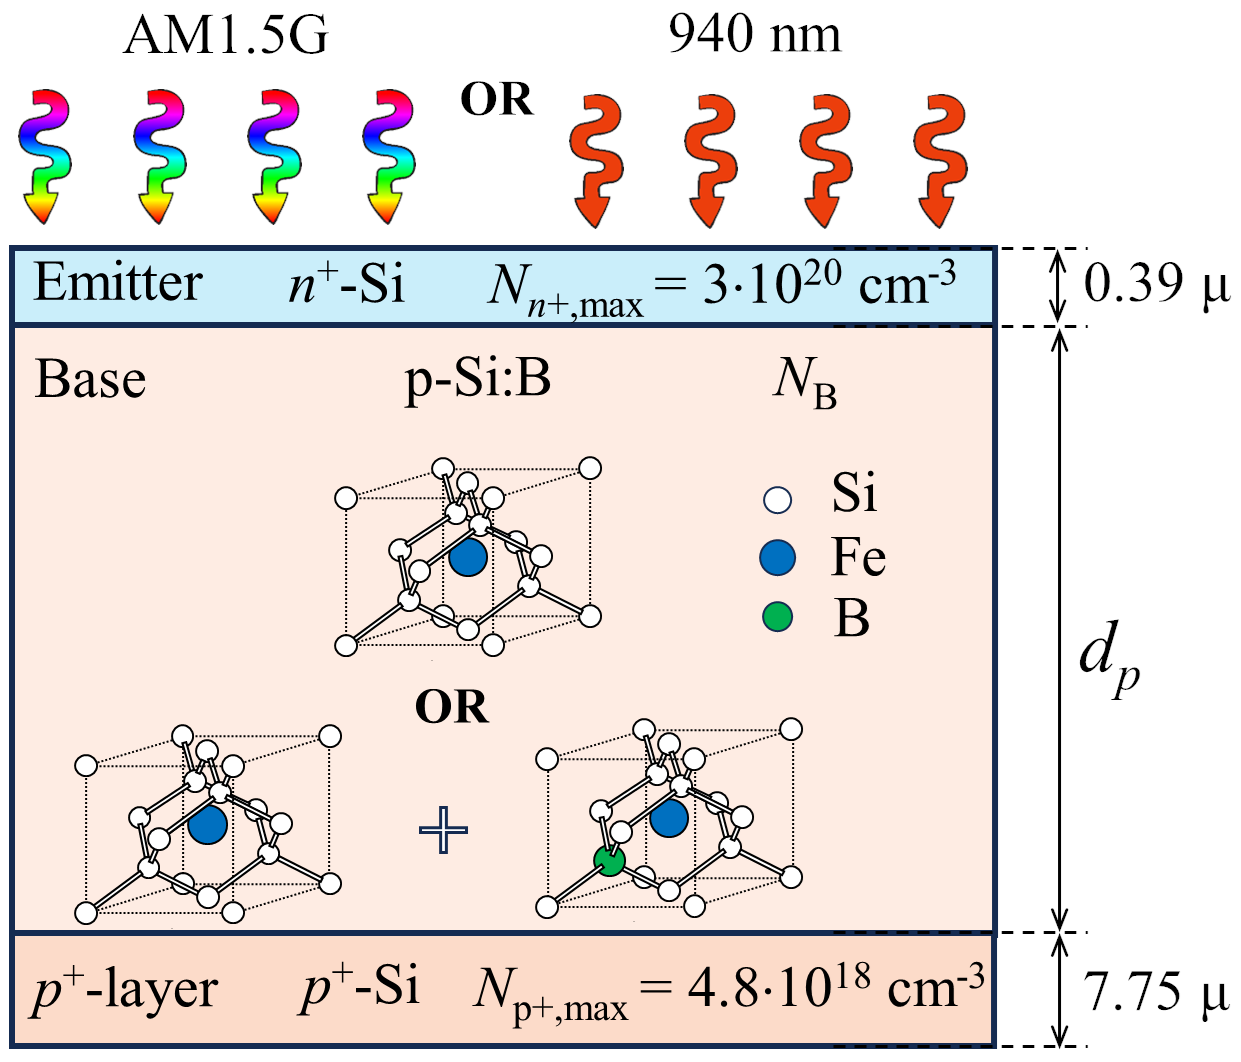
\includegraphics[width=0.5\linewidth]{Figure1.png}
	  \caption{Schematic diagram of analyzed solar cells.}\label{fig1}
\end{figure}


\begin{table}
\caption{Parameters varied during the simulation}\label{table1}
\begin{tabular*}{\tblwidth}{@{}LL@{}}
\toprule
  Parameter & Range of values \\ % Table header row
\midrule
 $d_p$($\mu$m)   & $180-380$\\
 $N_\mathrm{B}$ (cm$^{-3}$)    & $10^{15} - 10^{17}$\\
 $N_\mathrm{Fe}$ (cm$^{-3}$) & $10^{10} - 10^{14}$\\
 $T$ (K)                        & $290 - 340$\\
 Illumination                 & AM1.5G, 1000~W/$\mathrm{m}^{2}$; \\
 & 940~$\mathrm{nm}$, 5~W/$\mathrm{m}^{2}$; 940~$\mathrm{nm}$, 10~W/$\mathrm{m}^{2}$\\
\bottomrule
\end{tabular*}
\end{table}


The simulation was conducted using the SCAPS~3.3.11 code \cite{SCAPS1}.
SCAPS-1D software, developed by the University of Gent, is founded on theoretical computations that involve solving Poisson's equation,
continuity equations for holes and electrons, and drift-diffusion at each position within the solar cell,
considering the boundary conditions.
Despite its one-dimensional modeling approach, SCAPS is extensively used for modeling various types of solar cells \cite{Joshi2024,Ravidas2024,Liu2024,You2023} in general
and for investigating the effects of defects on their performance \cite{AitAbdelkadir2023,Liang2024,SCAPSDefect3} in particular.


As can be seen from Table~\ref{table1}, calculations spanned a broad range of temperatures and base doping levels.
Therefore, to improve the accuracy of the calculations when inputting the initial parameters into SCAPS,
temperature and concentration (where applicable) dependencies of the following silicon parameters were taken into account:

\begin{itemize}
    \item bandgap according to Passler \cite{Passler2002};
    \item doping induced bandgap narrowing according to Yan \& Cuevas \cite{EgNarrow};
    \item effective density of states at conduction and valence band and intrinsic carrier concentration according to Couderc et al. \cite{Si_ni_Couderc};
    \item thermal carrier velocities according to Green \cite{Nc:Green};
    \item free carrier effective masses according to O’Mara et al. \cite{OMara};
    \item carrier mobilities according to Klaassen's theory \cite{KLAASSEN953};
\end{itemize}

The values of surface recombination coefficients were considered equal to the thermal velocities of carriers \cite{Fell2015}.
The calculations addressed recombination processes within the structural volume,
incorporating both intrinsic recombination and Shockley-Read-Hall recombination at iron-related defects.
In the first case, processes of band-to-band radiation recombination were considered
(where the calculation of the corresponding coefficient included the fraction of radiatively emitted photons
reabsorbed via band-to-band processes according to Niewelt et al.\cite{Brad2022})
and Auger recombination (where the coefficients considered the effect of Coulomb enhancement \cite{AugerSi2022} and temperature dependence \cite{Si_Auger}).


When accounting for the influence of iron impurities,
we considered that Fe atoms were uniformly distributed within the base and $p^+$-layer
with a total concentration of $N_\mathrm{Fe}$ (see Table~\ref{table1}).
Two cases were under consideration:

Case~1.
The concentration of interstitial iron defects $\left[\mathrm{Fe}_i\right]=N_\mathrm{Fe}$  at each position throughout the solar cell,
with no pairs present $\left[\mathrm{Fe}_i\mathrm{B}_s\right]=0$.
This case corresponds to the state of the structure immediately after intense illumination, for example.

Case~2.
Iron atoms predominantly form pairs with acceptors, $\left[\mathrm{Fe}_i\mathrm{B}_s\right] \gg \left[\mathrm{Fe}_i\right]$,
but the exact concentration ratio depends on the position of the Fermi level and temperature \cite{FeB:kinetic,MurphyJAP2011}
and varies from point to point within the solar cell.
Further details about calculation of the concentration profiles of Fe$_i$B$_s$ and Fe$_i$ are provided in \cite{Olikh2022PPV,Olikh2019SM}.
This case corresponds to prolonged storage of the structure in darkness or under conditions of low-intensity ($< 0.01$~J~cm$^{-2}$ \cite{Macdonald2004}) illumination.


During the calculations, it was assumed that Fe$_i$ forms a single donor level,
while the Fe$_i$B$_s$ pair has a trigonal configuration and acts as an amphoteric defect.
We obtained defect parameters (including level positions within the bandgap and electron and hole capture cross-sections) from relevant studies \cite{ROUGIEUX2018,Istratov1999}.

As previously mentioned, the solar cell behavior was simulated under different illumination conditions,
including solar light (AM1.5G) and monochromatic light (wavelength 940~nm, intensity of $W_\mathrm{ill} = 5$~Wm$^{-2}$ or 10~W/$\mathrm{m}^{2}$) --– see Table~\ref{table1}.
The calculations incorporated the light absorption values in silicon based on Green's study \cite{Green2022}.


The $I$-$V$ characteristics were simulated for both Case~1 and Case~2 (see Fig.~\ref{fig2}),
and from each curve, the short-circuit current, open-circuit voltage, efficiency, and fill factor were determined.
Assessing the influence of iron defect variability relied on the relative changes in each photovoltaic conversion parameter:

\begin{figure}
	\centering
		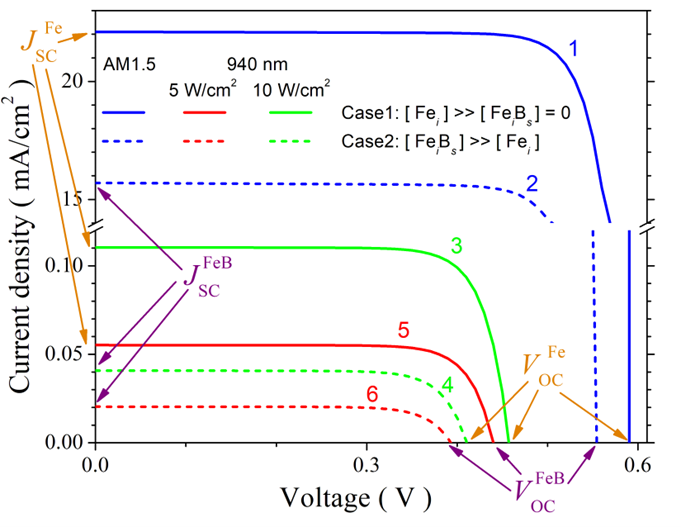
\includegraphics[width=0.5\linewidth]{Figure2.png}
	  \caption{Typical IV characteristics,
   calculated for structure with $d_p = 180$~$\mu$m, $N_\mathrm{B}=10^{17}$~cm$^{-3}$,
   $N_\mathrm{Fe}=10^{14}$~cm$^{-3}$ at $T = 290$~K.
   Illumination: AM1.5 (curves 1, 2), 940~nm 10~Wcm$^{-2}$ (3, 4) and 940~nm 5~Wcm$^{-2}$ (5, 6).
   Solid and dotted lines correspond to Case~1 and Case~2, respectively.}\label{fig2}
\end{figure}


\begin{equation}
    \varepsilon A = \frac{A^\mathrm{FeB} - A^\mathrm{Fe}}{A^\mathrm{FeB}} \times 100 \%\,,
\end{equation}
where $A$ represents one of the parameters ($I_\mathrm{SC}$, $V_\mathrm{OC}$, $\eta$, and $FF$),
superscript ‘‘FeB’’ corresponds to the parameter value for coexistence of Fe$_i$ and Fe$_i$B$_s$ (Case~2),
superscript ‘‘Fe’’ is related to the decay of all pairs (Case~1).


Impact of change of iron defects was investigated as a function of temperature from 290~K to 340~K,
base depth from 180~$\mu$m to 380~$\mu$m,
base doping level from $10^{15}$~cm$^{-3}$ to $10^{17}$~cm$^{-3}$,
and total impurity iron atom concentration from $10^{10}$~cm$^{-3}$ to $10^{14}$~cm$^{-3}$.
For each illumination scenario, calculations were carried out with 11 different temperature values and 5 base depth values,
evenly distributed within the specified ranges.
The concentration values were distributed equally on a logarithmic scale with 4 ($N_\mathrm{B}$ case) and 6 ($N_\mathrm{Fe}$ case) steps per decade.
As a result, for the AM1.5 illumination scenario, for instance, 24750 $I$-$V$ characteristics were simulated.
An exception occurred with monochromatic illumination at $W_\mathrm{ill} = 10$~Wm$^{-2}$,
where we used only two $d_p$ values.

\subsection{Experimental Details}

To evaluate the validity of the simulated results,
we also conducted experimental studies on the effect of changing the state of iron-related defects on the photoelectric parameters of silicon solar cells.

The $n^+$-$p$-$p^+$-Si samples were used in the experiment.
The structure was fabricated from a 380~$\mu$m thick $p$-type boron-doped
Czochralski silicon (100) wafer with doping level $N_\mathrm{B}=1.36\times10^{15}$~cm$^{-3}$.
The $n^+$ emitter with a sheet resistance of about $20-30$~$\Omega/\Box$
and  thickness of $0.7$~$\mu$m was formed by phosphorus diffusion.
The anti-recombination isotype barrier was created by using a $p^+$
layer ($10-20$~$\Omega/\Box$) formed by boron diffusion.
On the front surface, SiO$_2$ (40~nm) and Si$_3$N$_4$ (30~nm) films were formed as antireflective and passivating layers, respectively.
The solid and grid Al contacts were formed by magnetron sputtering on the back and front surfaces, respectively.

The $I$-$V$ characteristics were measured using a Keithley 2450 source meter and
low--intensity monochromatic light source (light--emitting diode SN--HPIR940nm--1W with light wavelength 940~nm and intensity of about  $W_\mathrm{ill} = 5$~Wm$^{-2}$).

For different samples, the iron concentration ranged from $2\times10^{11}$ to $4\times10^{13}$~cm$^{-3}$.
The values of $N_\mathrm{Fe}$ were determined using a methodology \cite{Olikh2022:JMatSci,Olikh2021JAP}, based on fitting the kinetics of short-circuit current.
The decay of Fe$_i$B$_s$ pairs was realized using intensive (7000~W/$\mathrm{m}^{2}$) halogen lamp illumination.

The measurements were carried over the temperature range of 300-340~K.
The sample temperature was driven by a thermoelectric cooler controlled by an STS-21 sensor
and maintained constant by a PID algorithm embedded in the software that serves the experimental setup.


\section{Results and Discussion}%\label{}

\subsection{Short--circuit current}


\begin{figure}
	\centering
     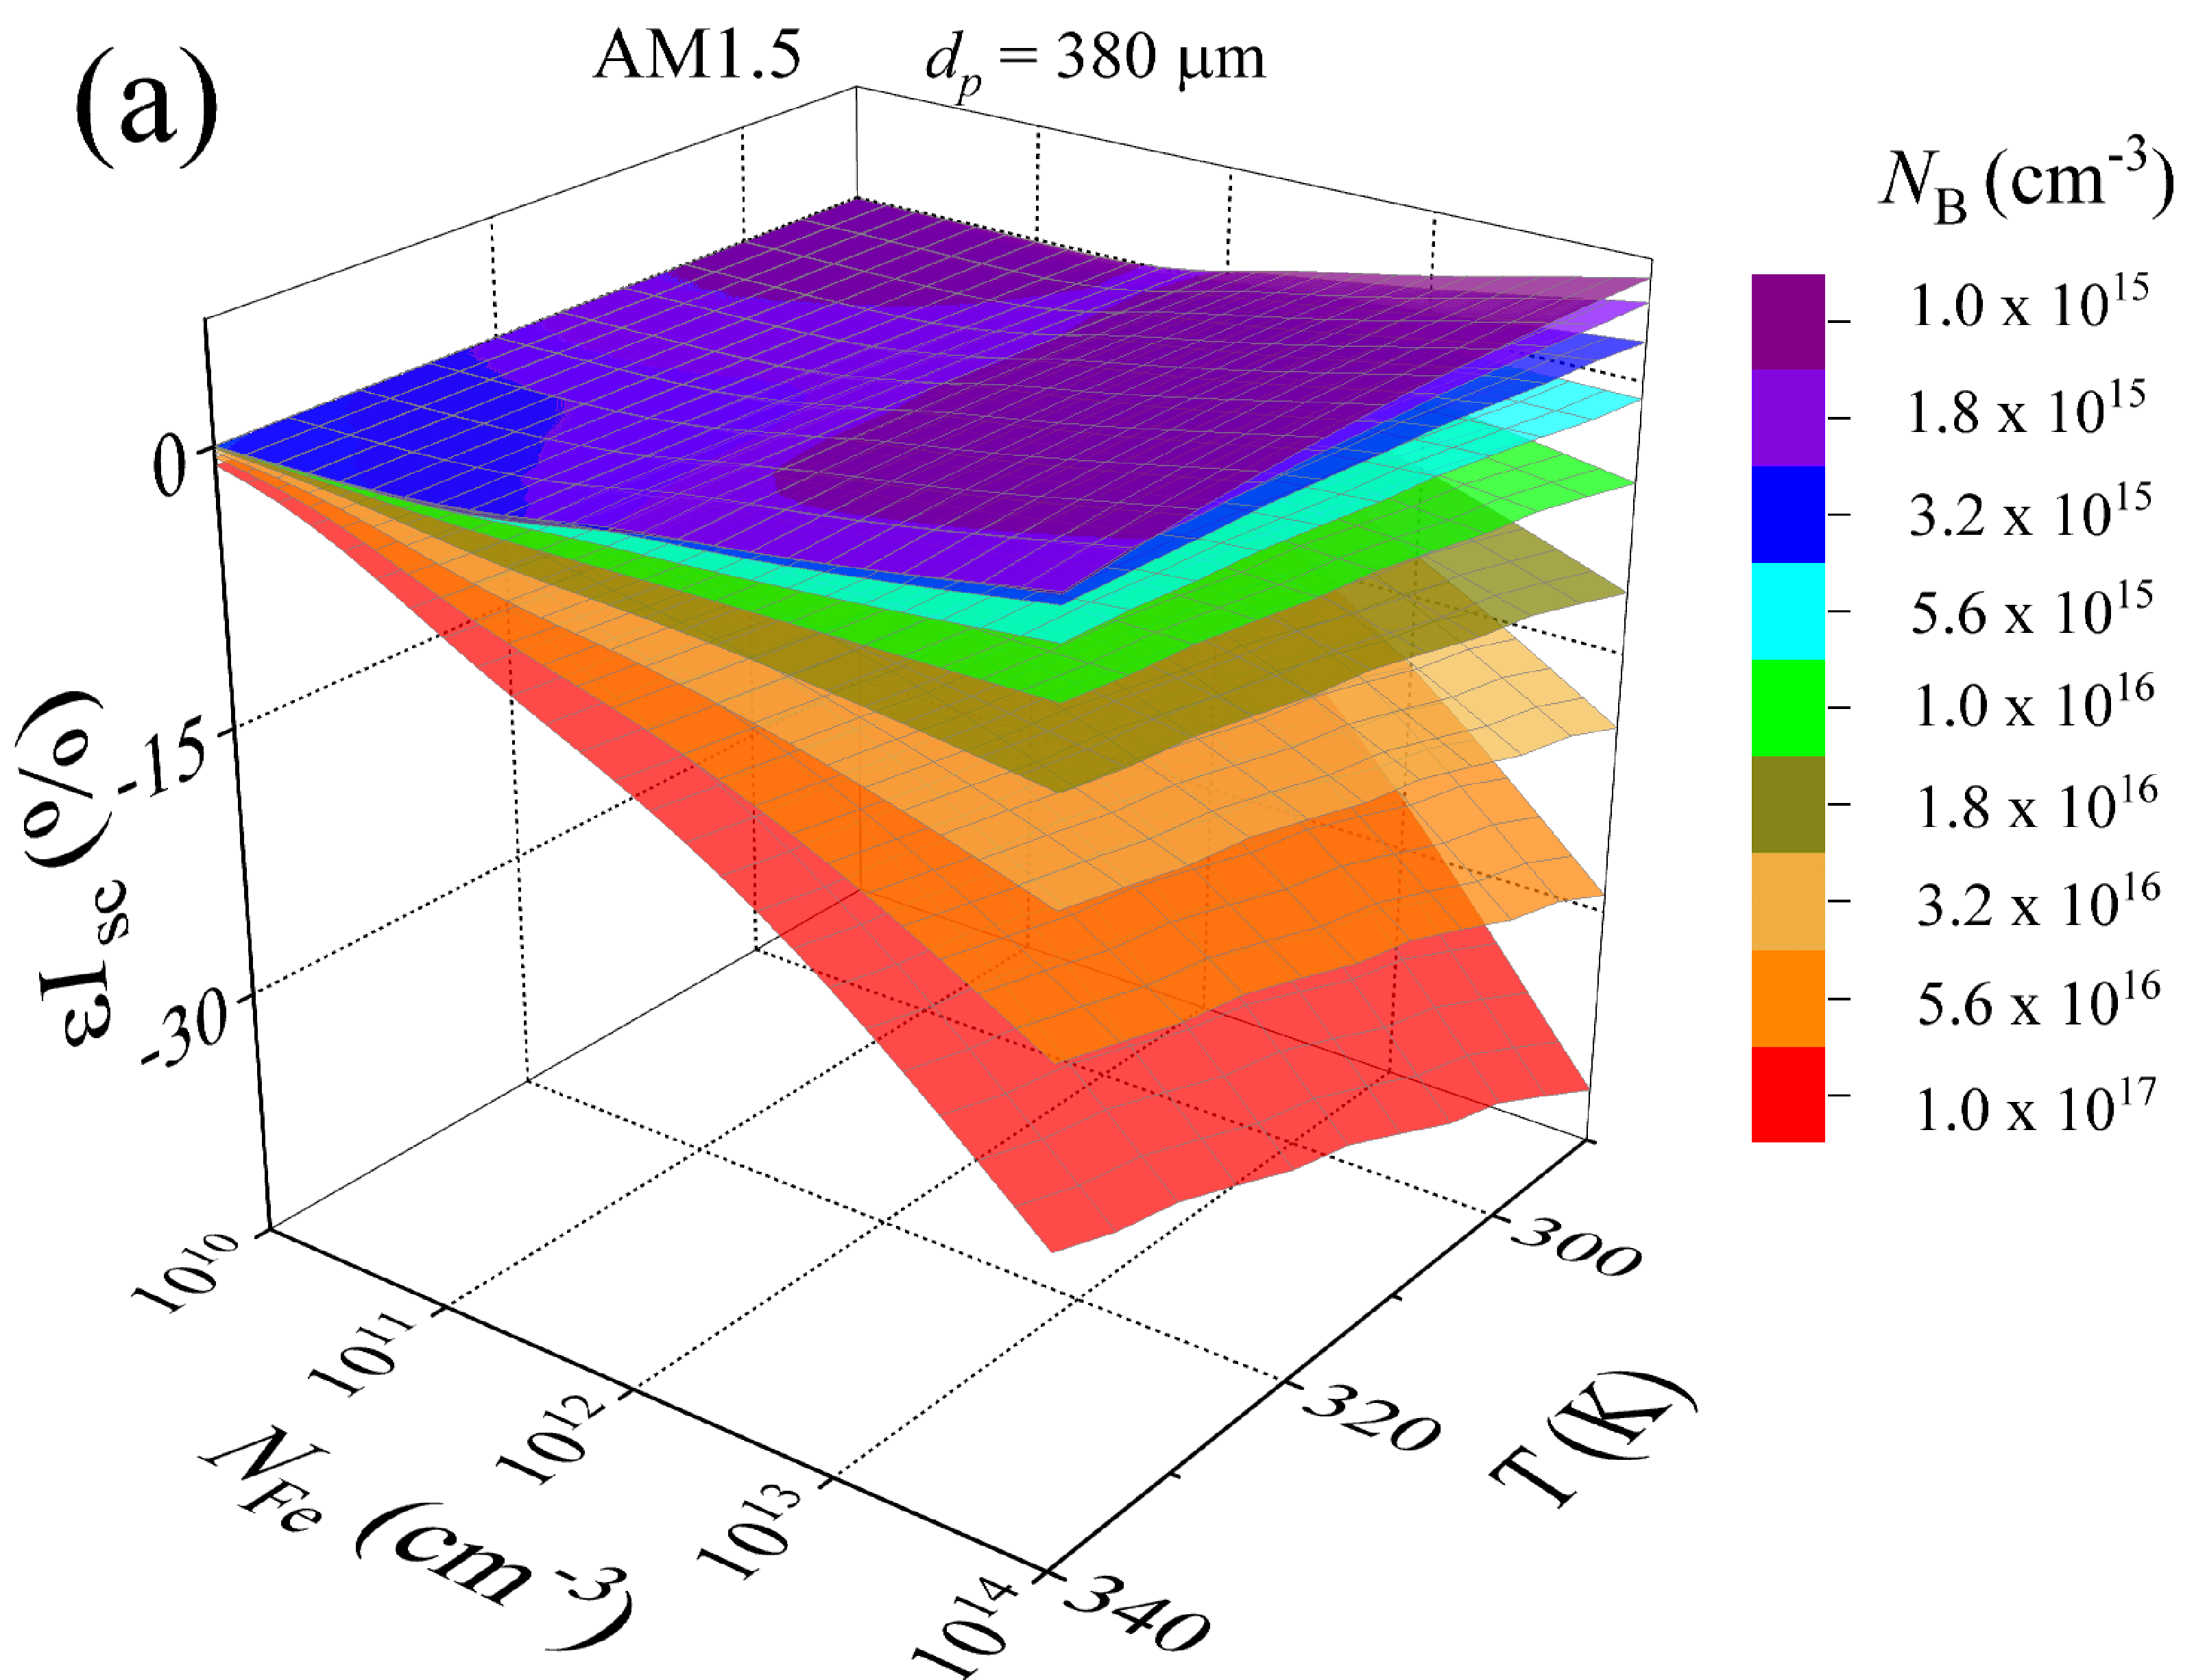
\includegraphics[width=0.49\linewidth]{Fig3a.png}
     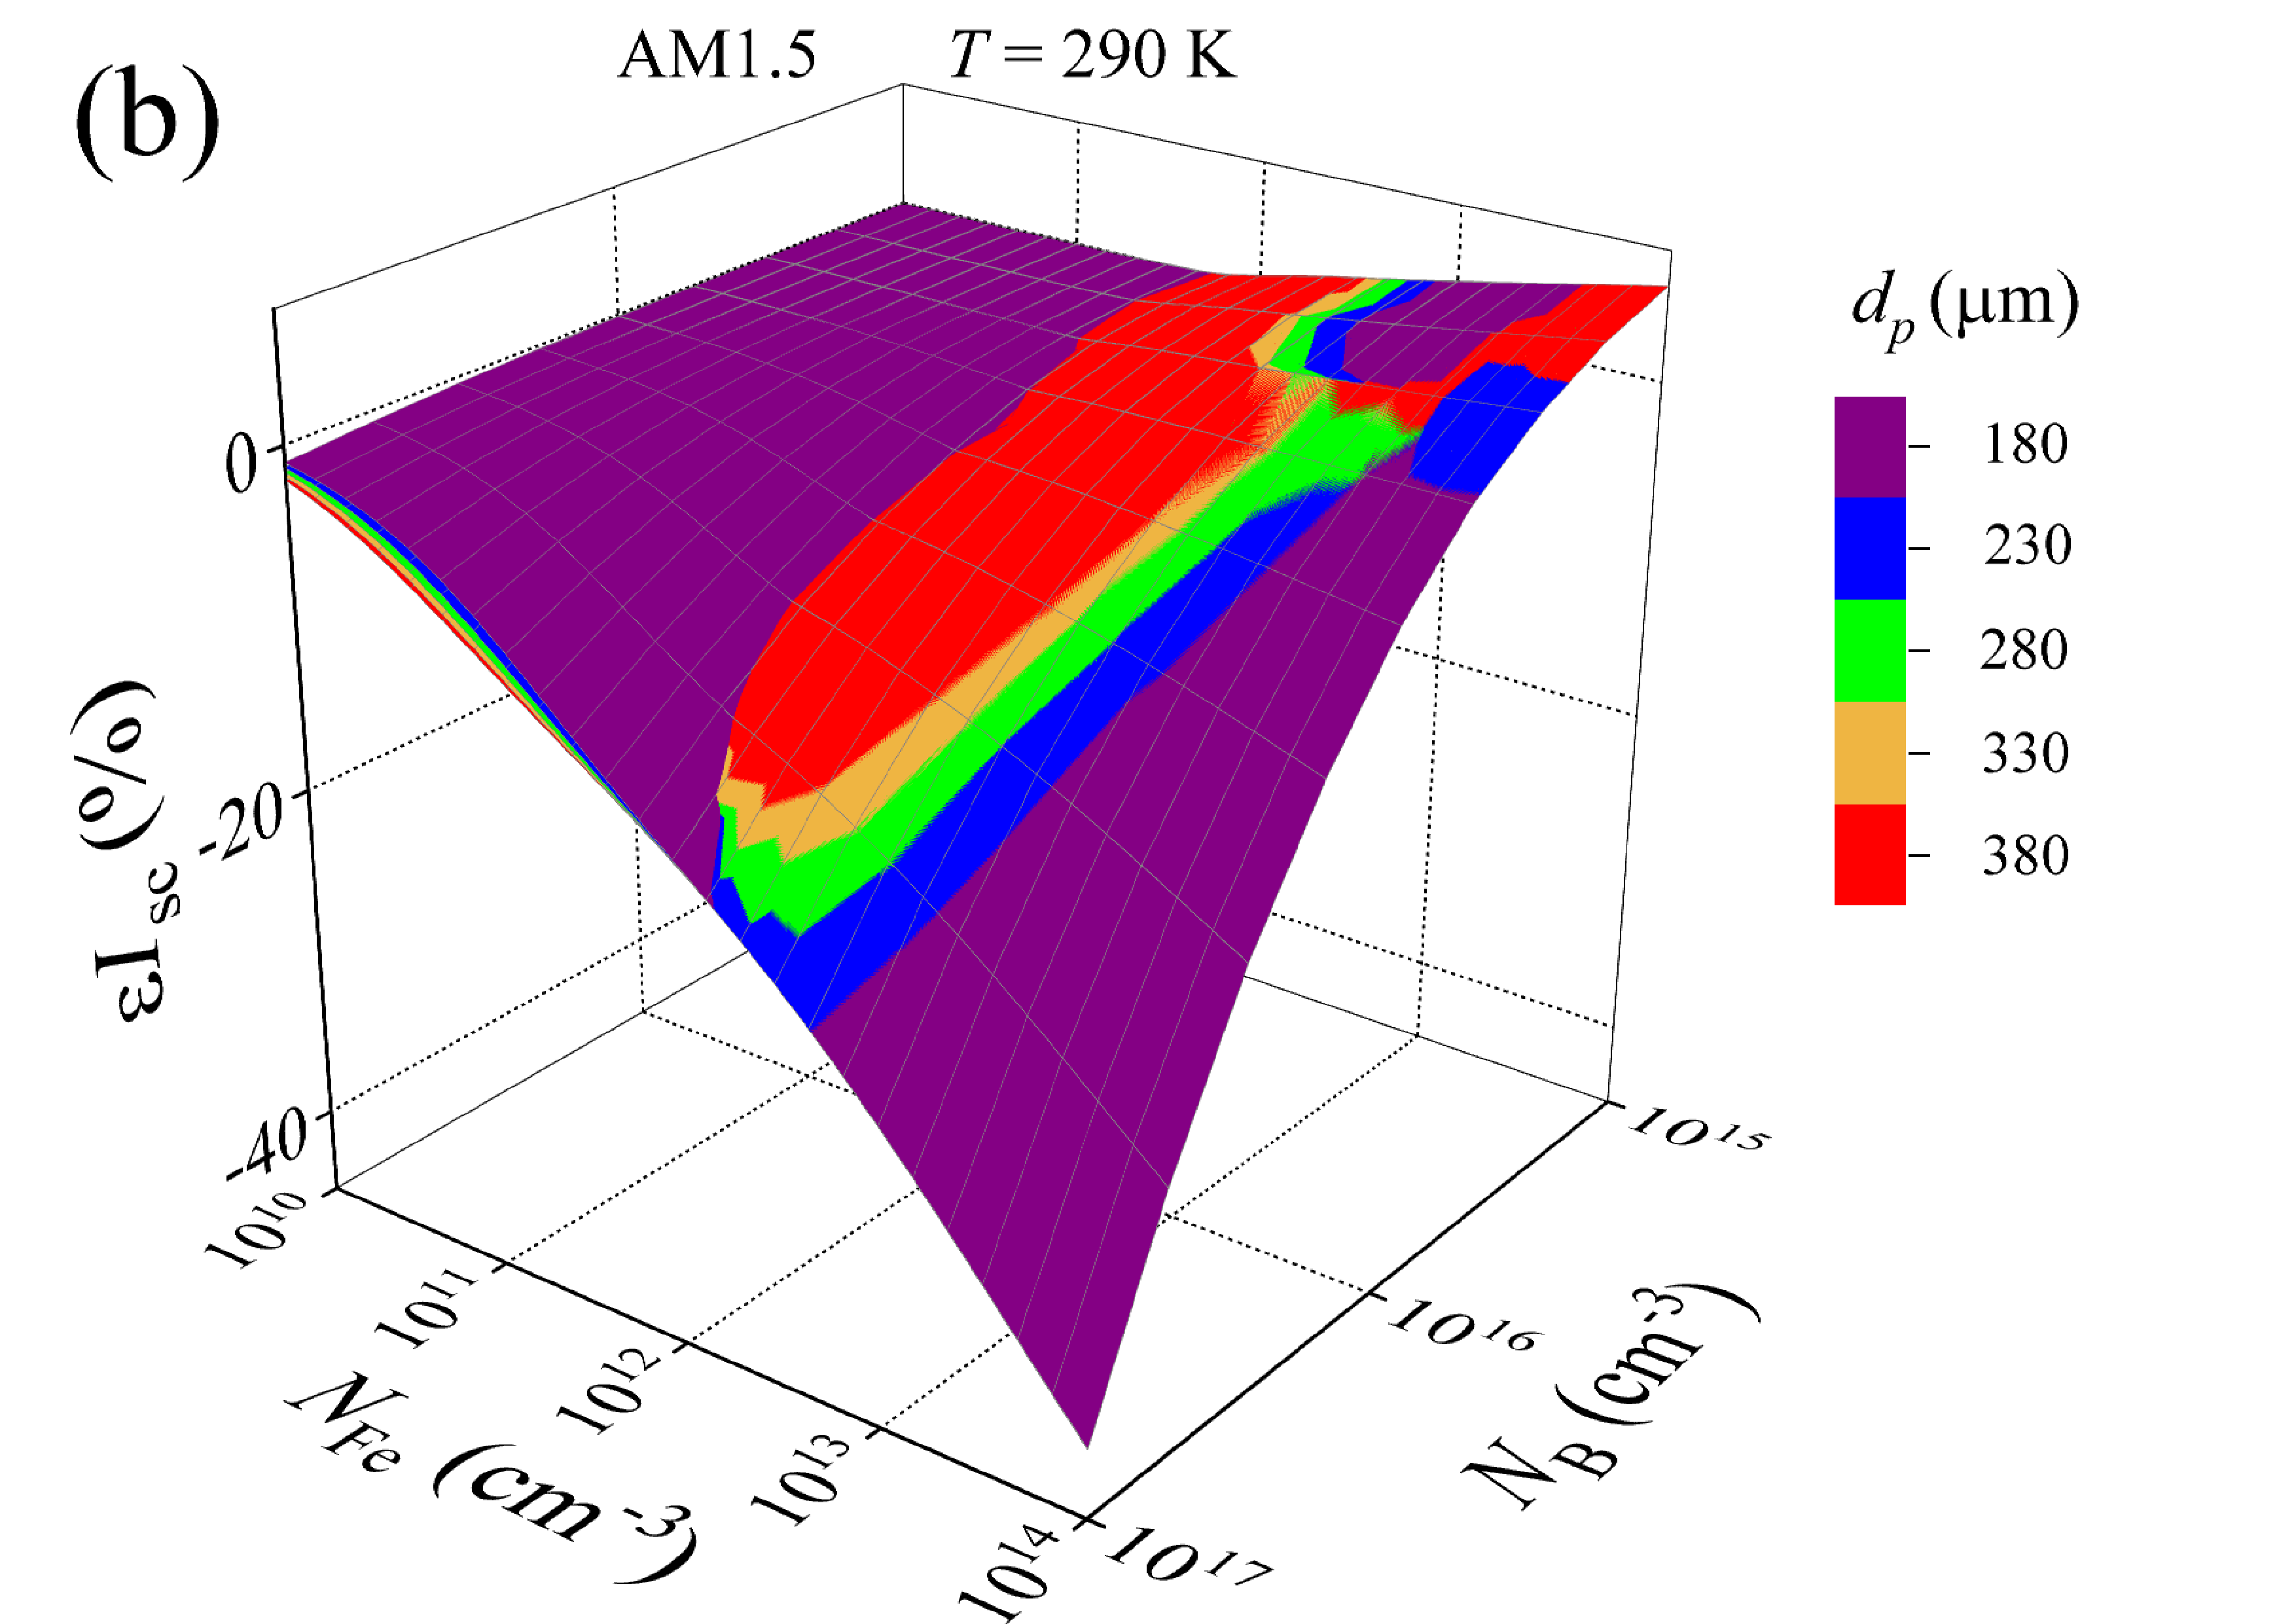
\includegraphics[width=0.49\linewidth]{Fig3b.png}
     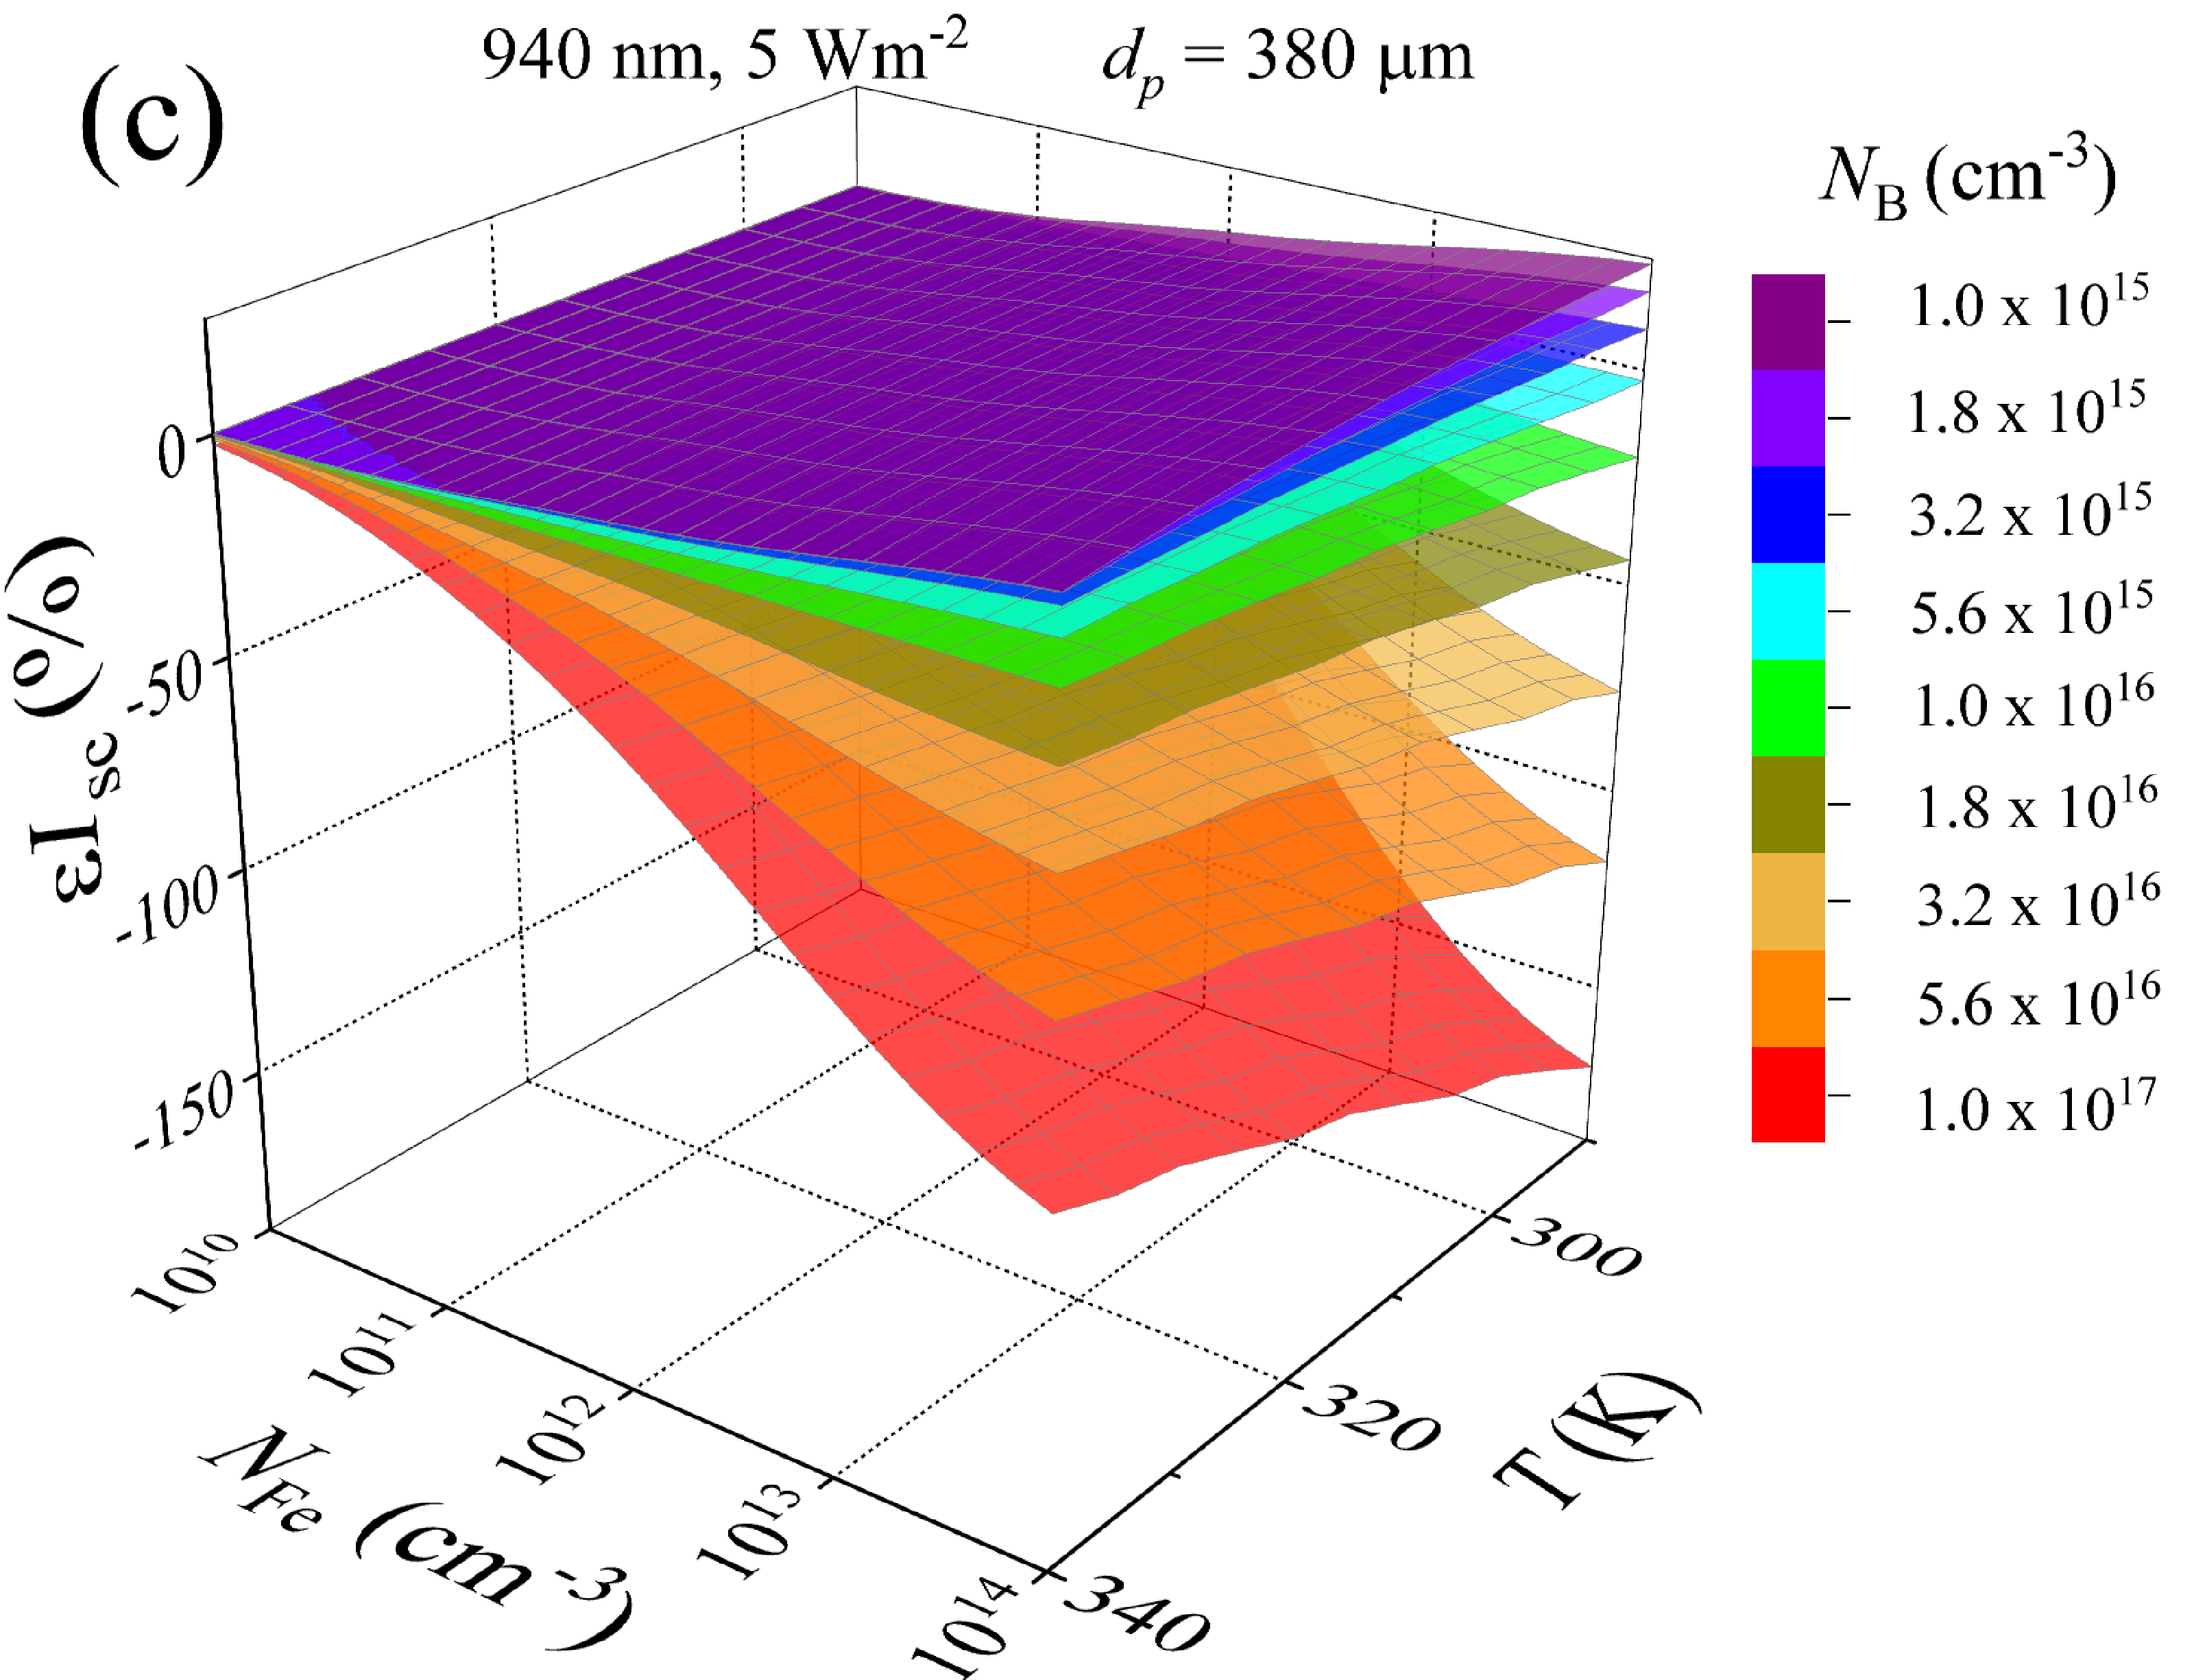
\includegraphics[width=0.49\linewidth]{Fig3c.png}
     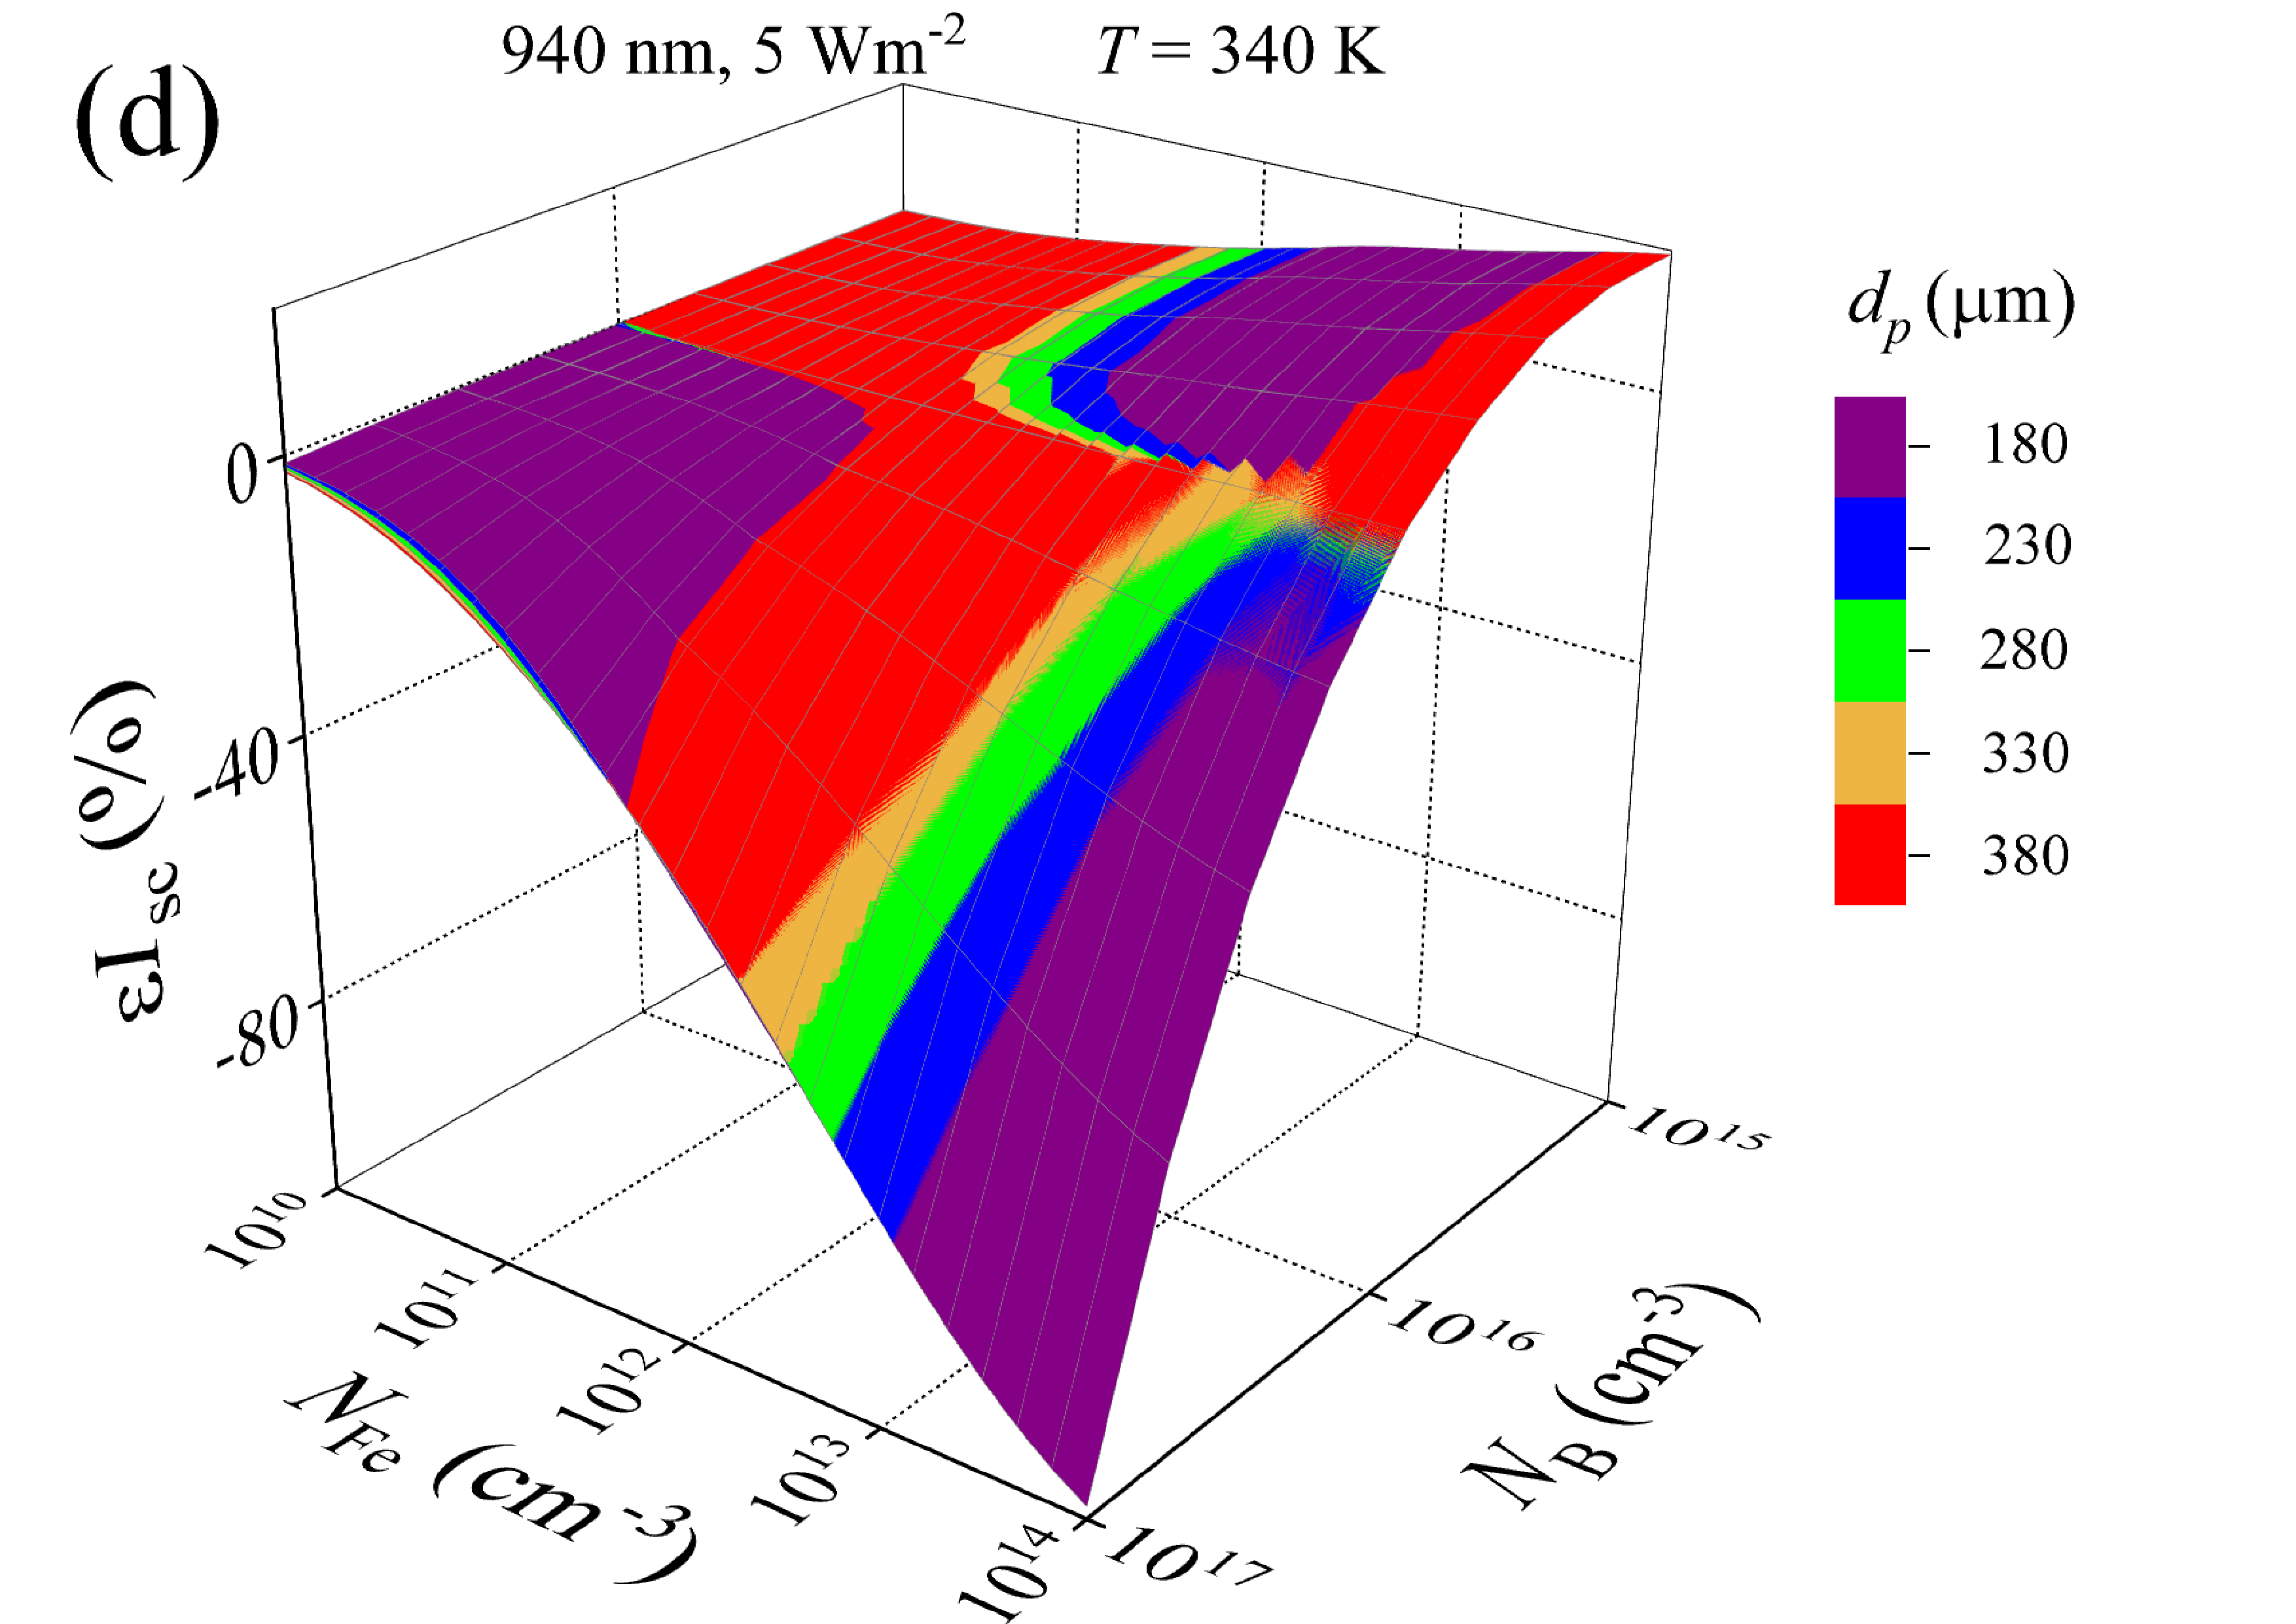
\includegraphics[width=0.49\linewidth]{Fig3d.png}
	  \caption{Dependencies of relative changes of short-circuit current on iron concentration and
       temperature (panels a and c) or doping level (b, d).
       Illumination: AM1.5 (a, b), 940~nm 5~Wm$^{-2}$ (c, d).
       $T$, K: 290 (b), 340 (d).
       Different surfaces correspond to different doping levels (a, c) and base depths (b, d).
}\label{fig3}
\end{figure}


\cite{YangHandbookPVSi,Goetzberger1998}

\begin{figure}
	\centering
     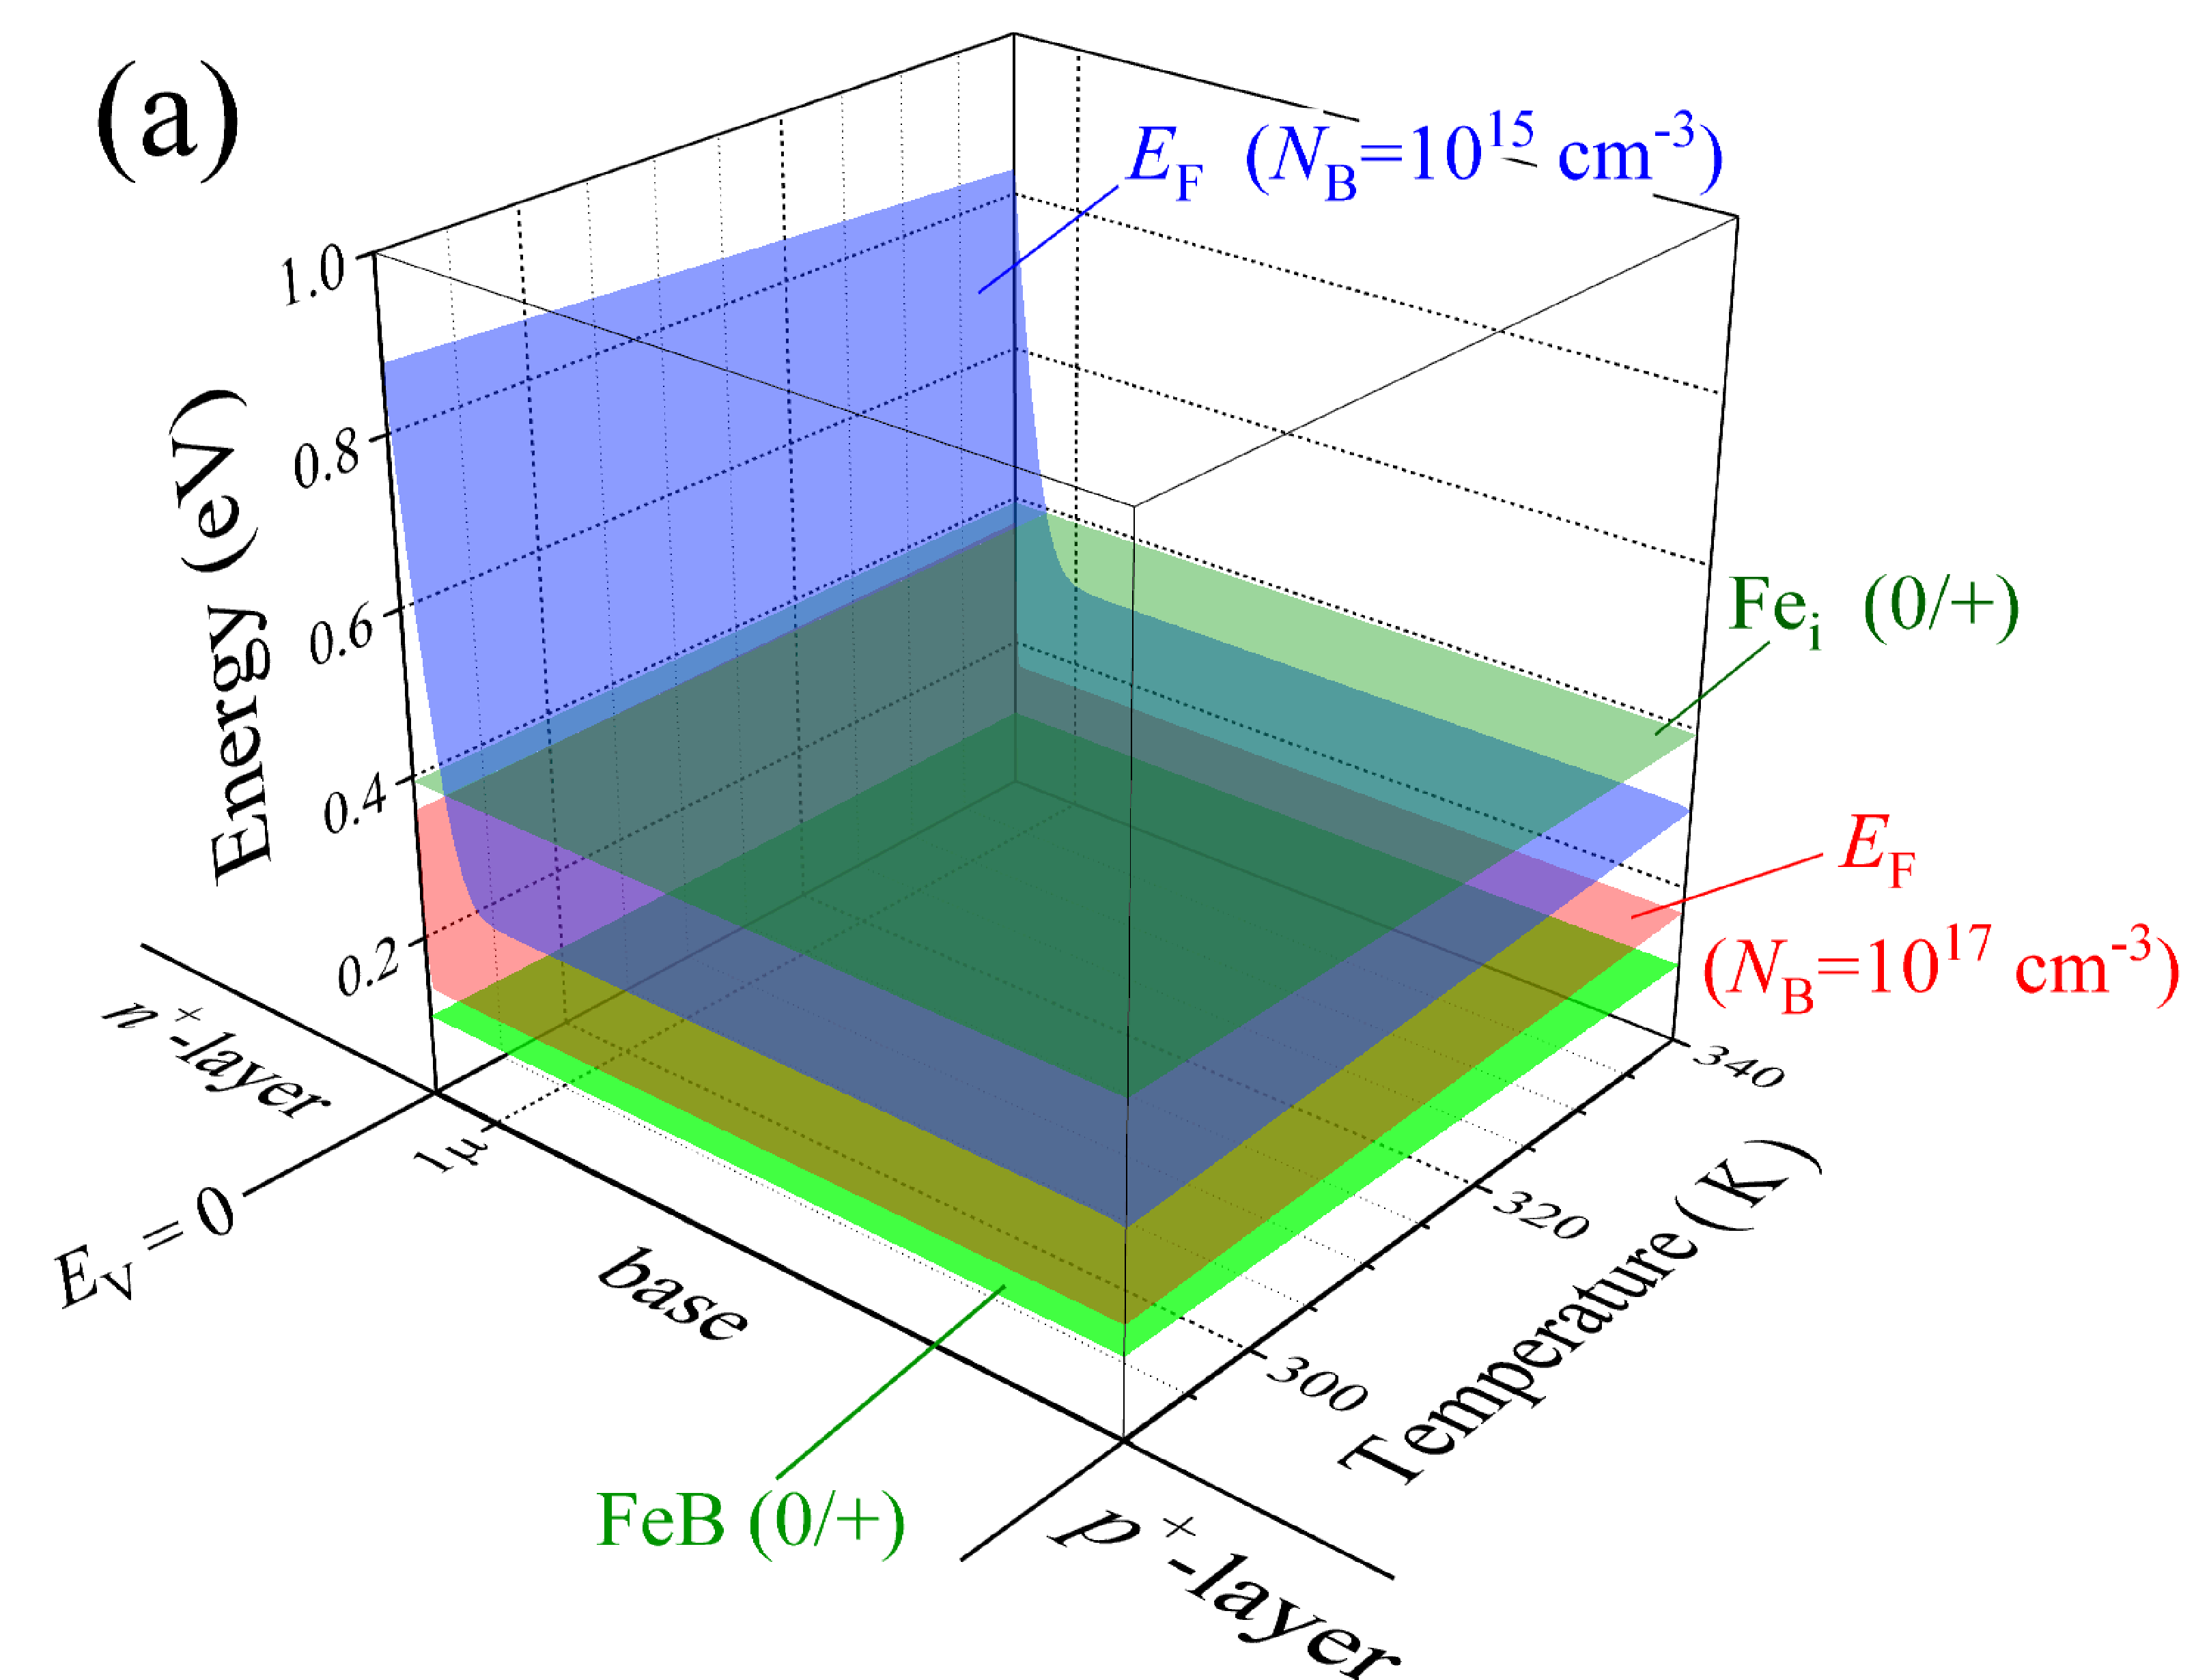
\includegraphics[width=0.49\linewidth]{Fig4a.png}
     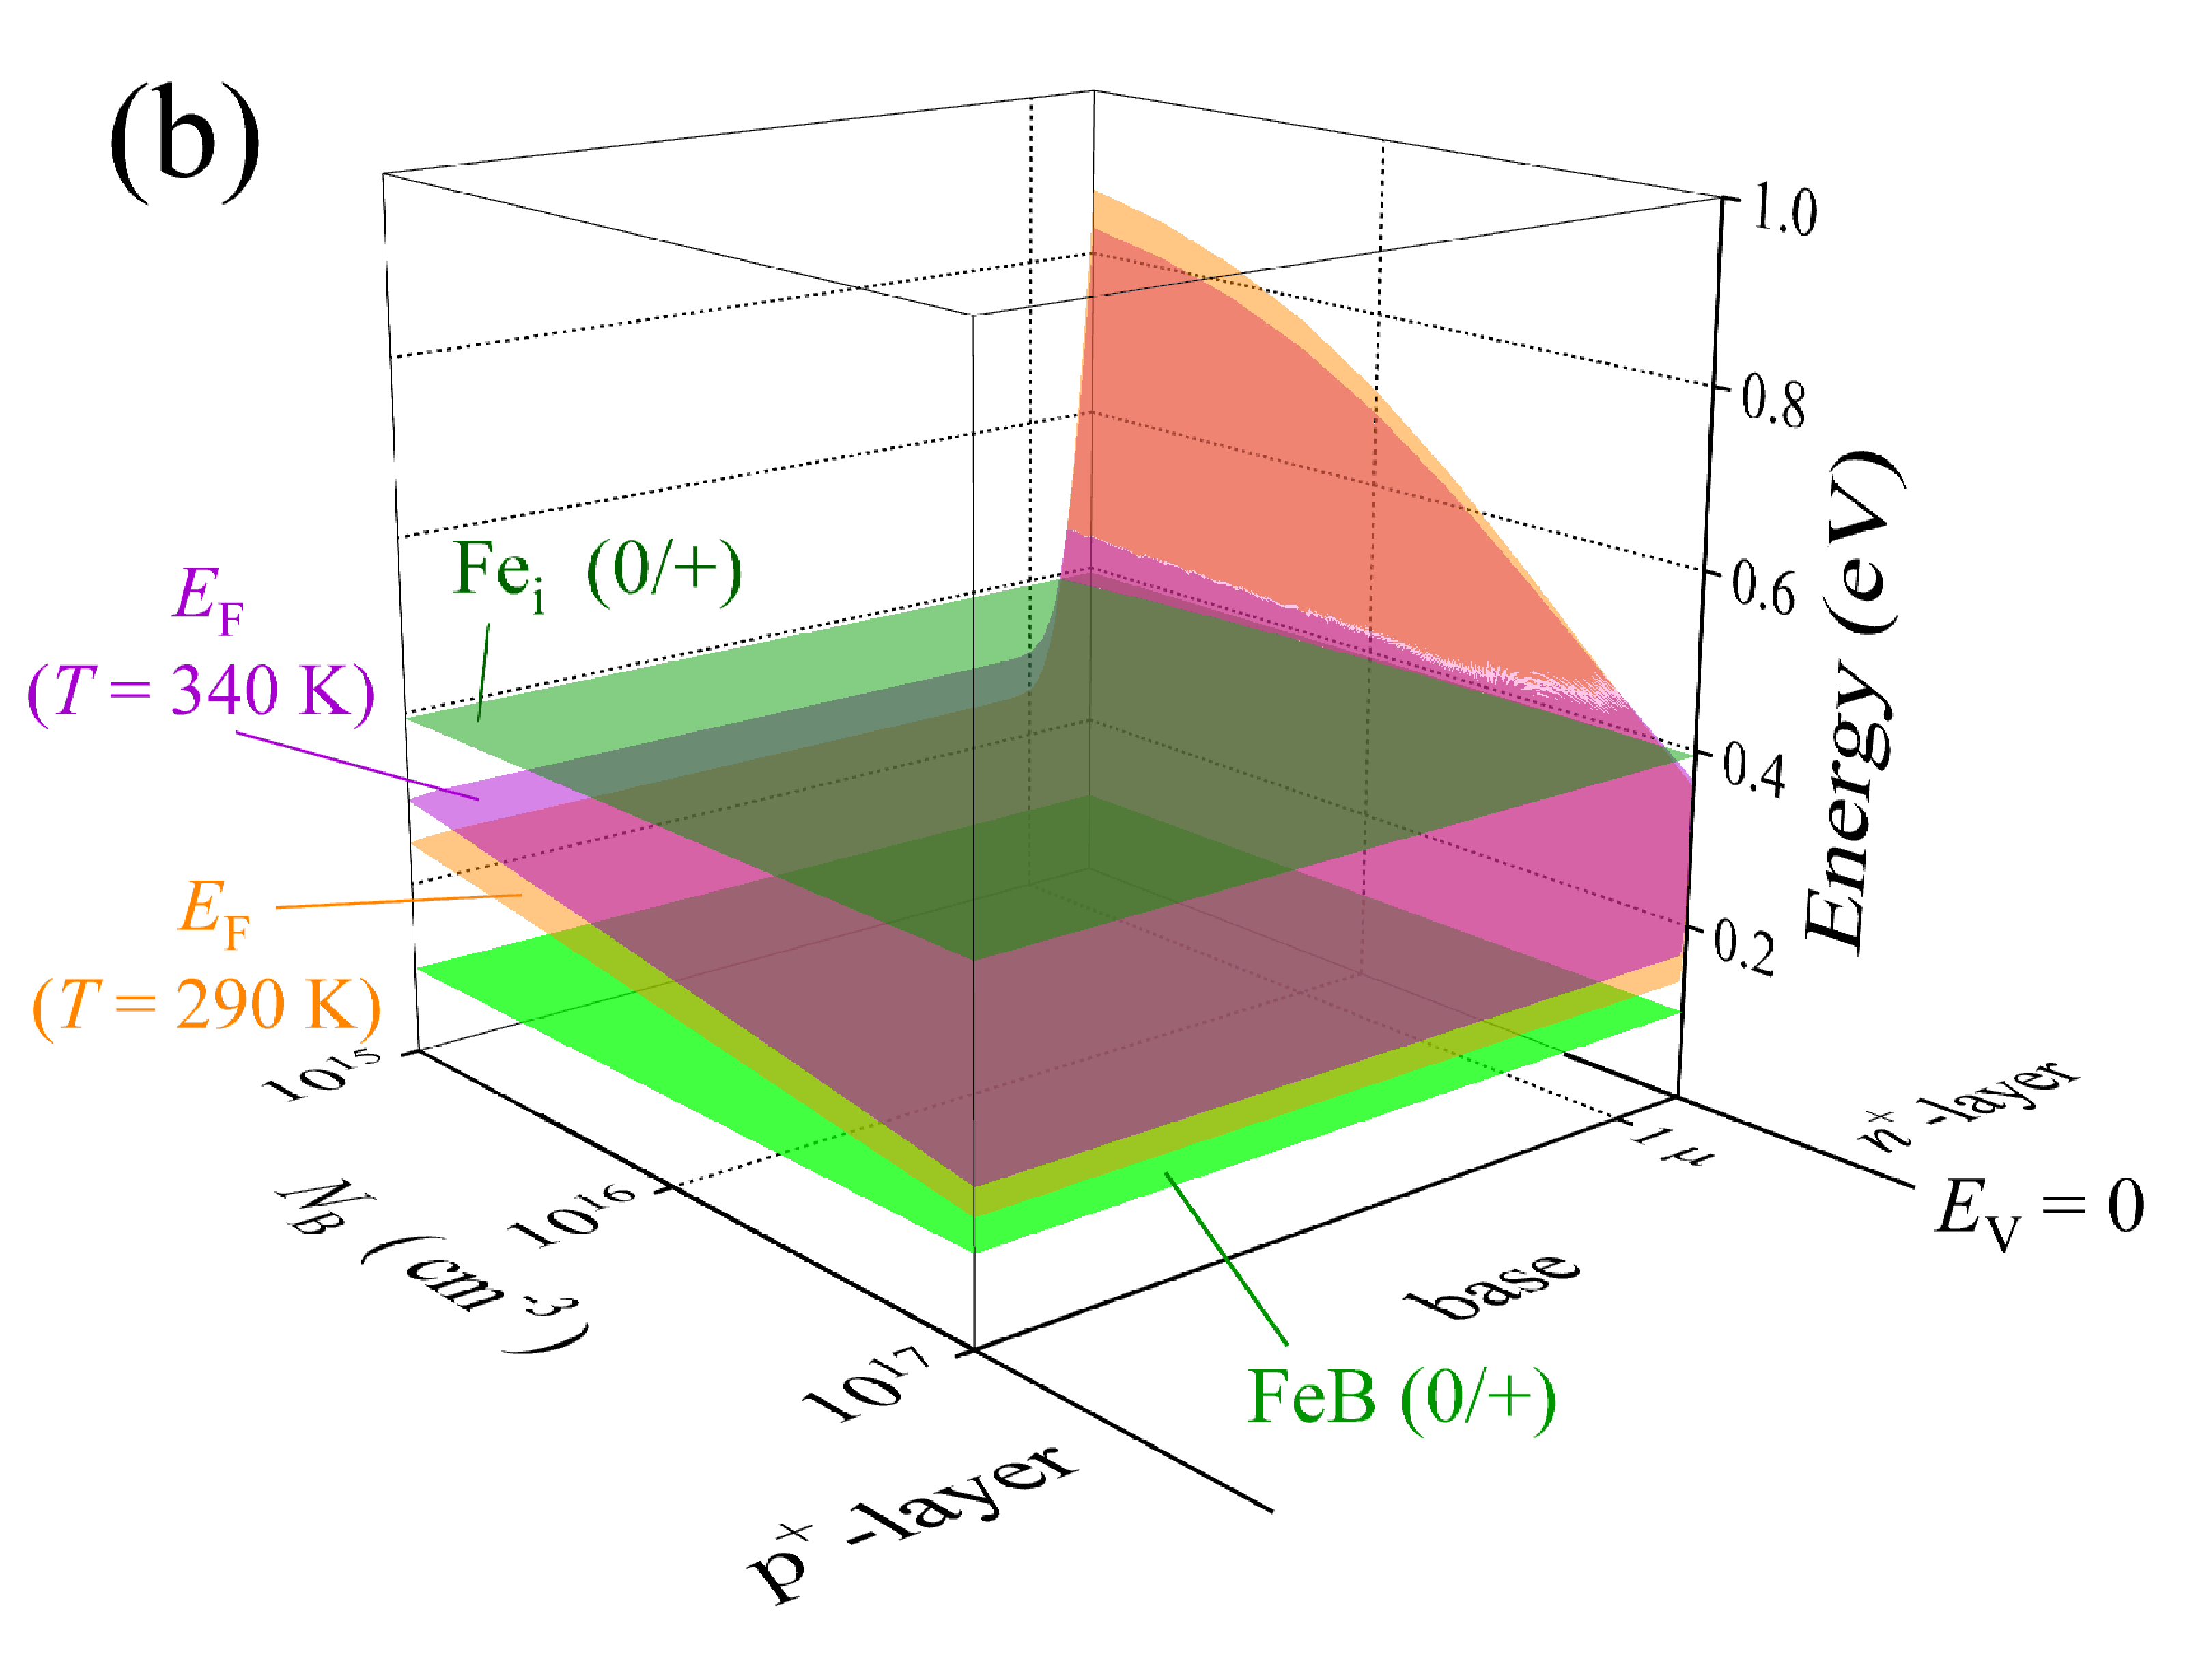
\includegraphics[width=0.49\linewidth]{Fig4b.png}
	  \caption{The location of the Fermi level in the base of the $n^+$-$p$-$p^+$ structure
       as a function of temperature for $N_\mathrm{B}=10^{15}$ and $10^{17}$~cm$^{-3}$ (a),
       and as a function of the doping level for $T=290$ and 340~K (b).
       The zero energy value corresponds to the top of the valence band.
       Also shown are the positions of the donor levels of the FeB pair (green surfaces)
       and the interstitial iron atom Fe$_i$ (olive surfaces).
}\label{fig4}
\end{figure}


\begin{figure}
	\centering
     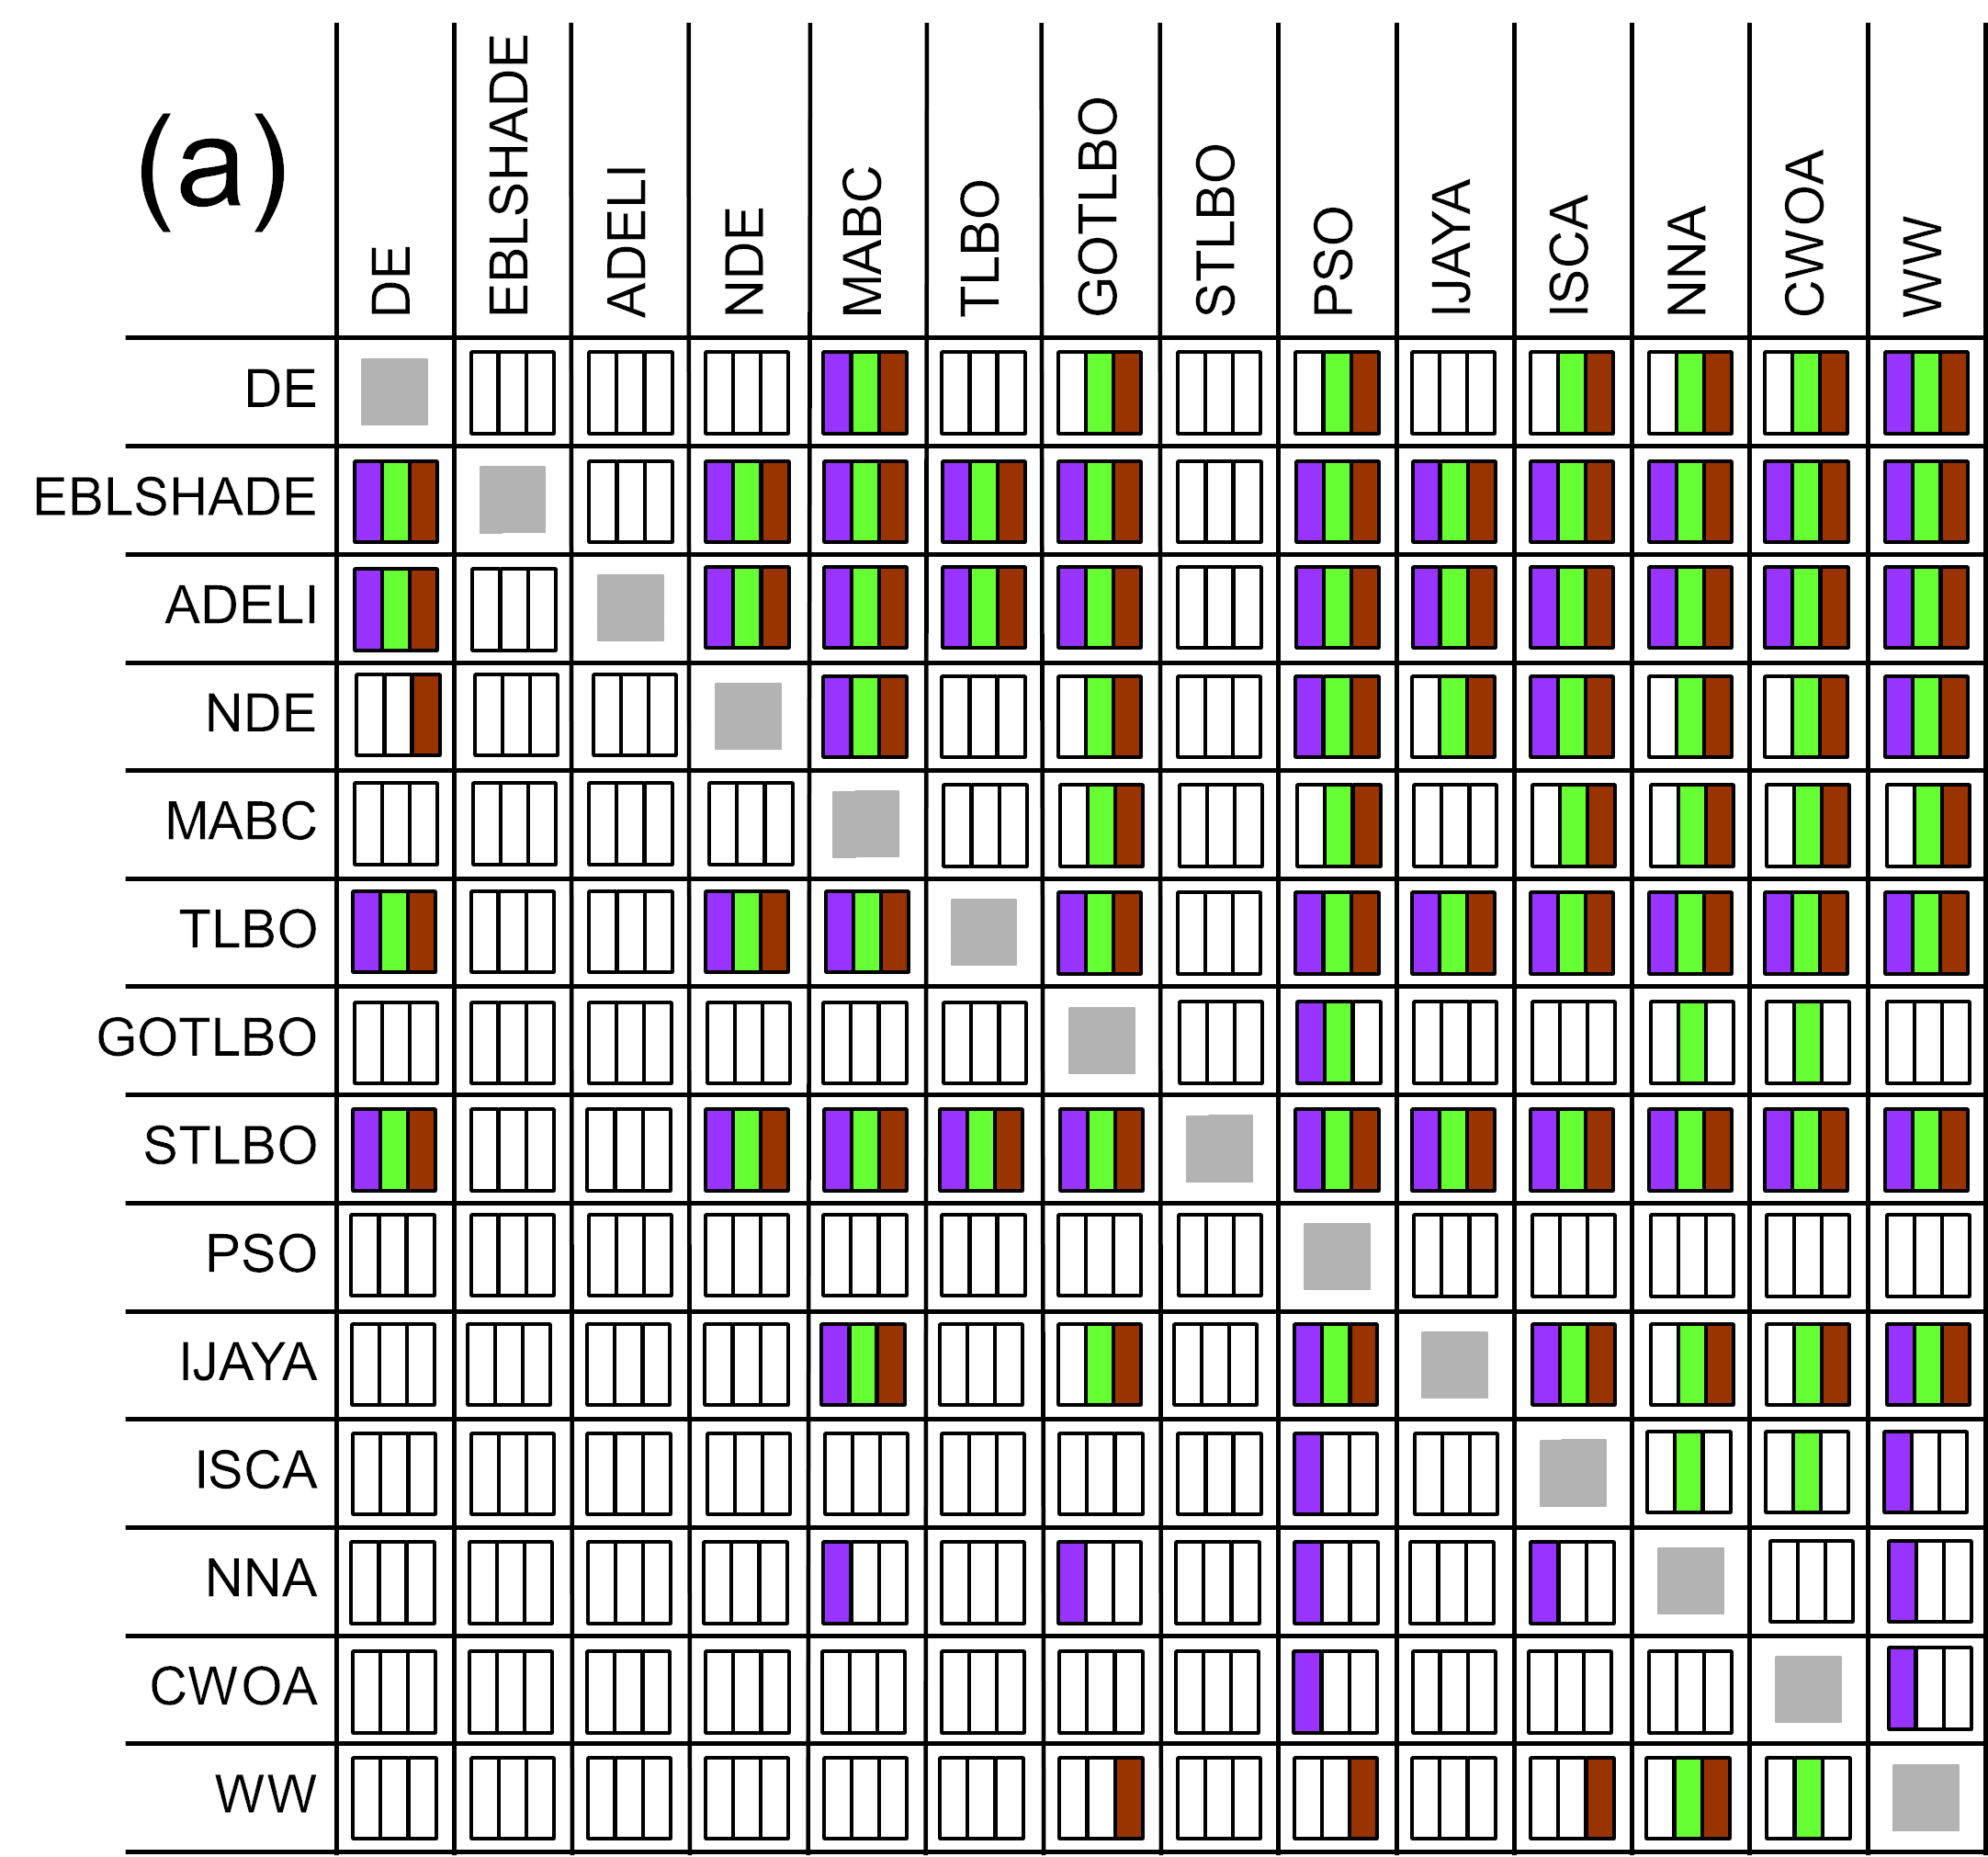
\includegraphics[width=0.4\linewidth]{Fig5a.png}
     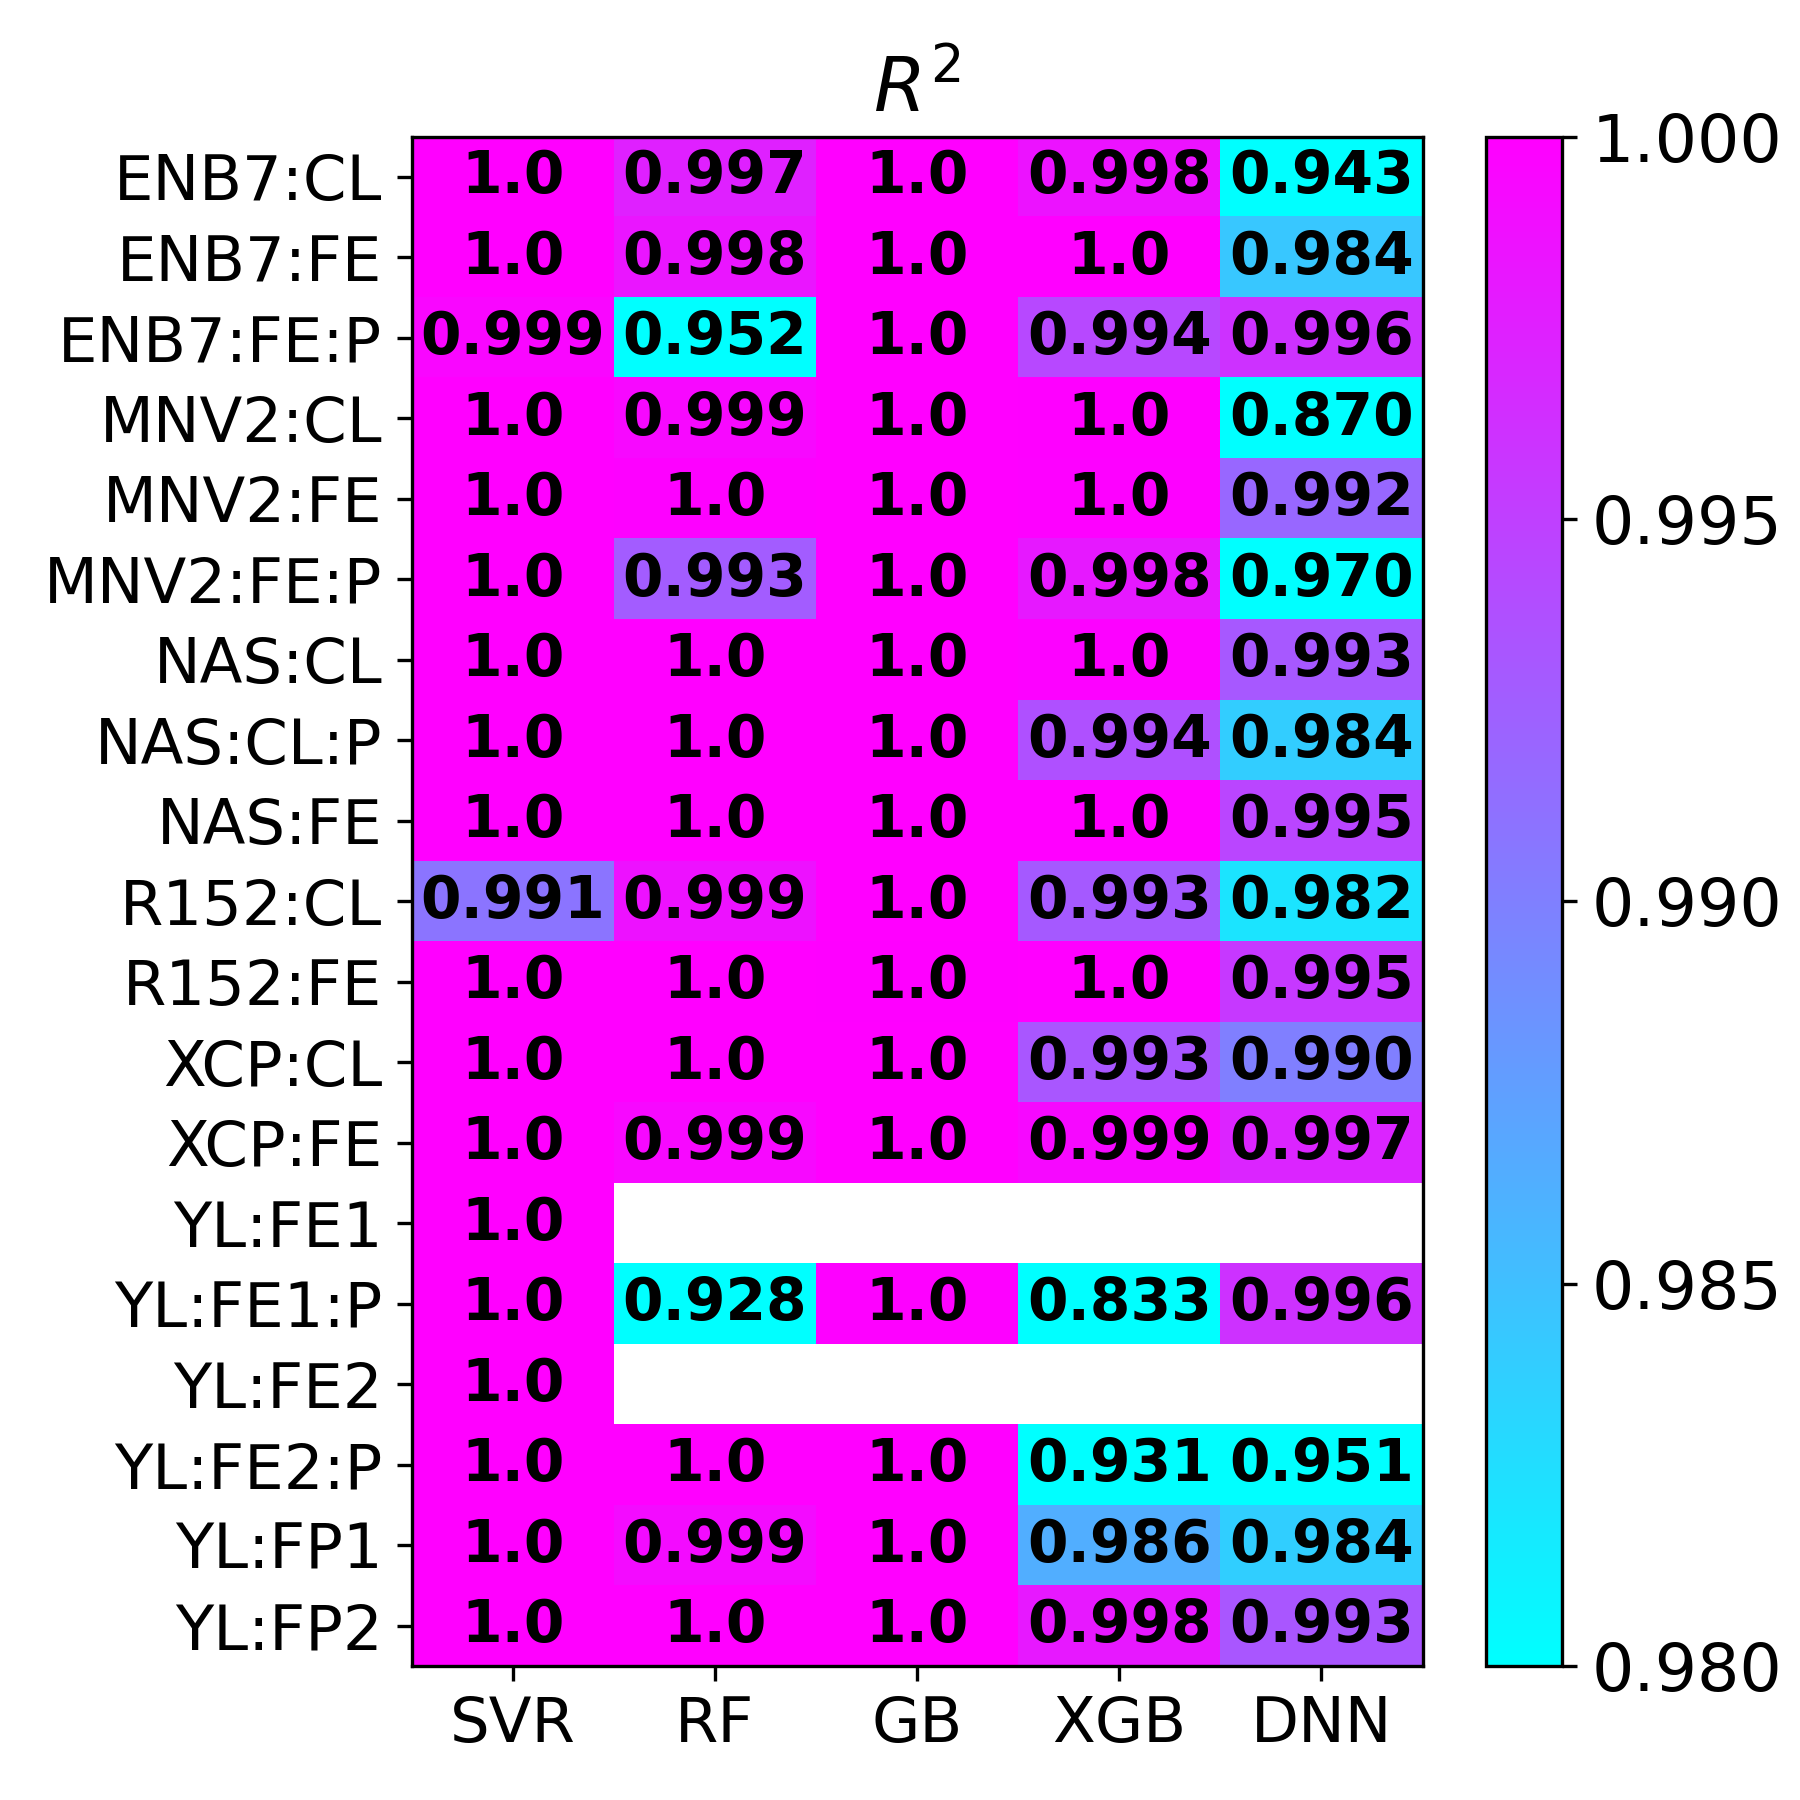
\includegraphics[width=0.4\linewidth]{Fig5b.png}
	  \caption{Dependencies of relative changes of short-circuit current on iron concentration (a) and
       temperature (b) for SSC with $d_p=380$~$\mu$m and $N_\mathrm{B}=1.36\times10^{15}$~cm$^{-3}$
       in the case of monochromatic (940~nm) illumination.
       The marks are the experimental results (divided by factor 1.4), the lines are the simulation results.
       $W_\mathrm{ill}$, Wm$^{-2}$: 5 (marks and solid lines), 10 (dotted lines).
       Different lines and marks correspond to different temperatures (a) or $N_\mathrm{Fe}$ values (b) --- see legends.
}\label{fig5}
\end{figure}

\subsection{Open-circuit voltage}

\begin{figure}
	\centering
     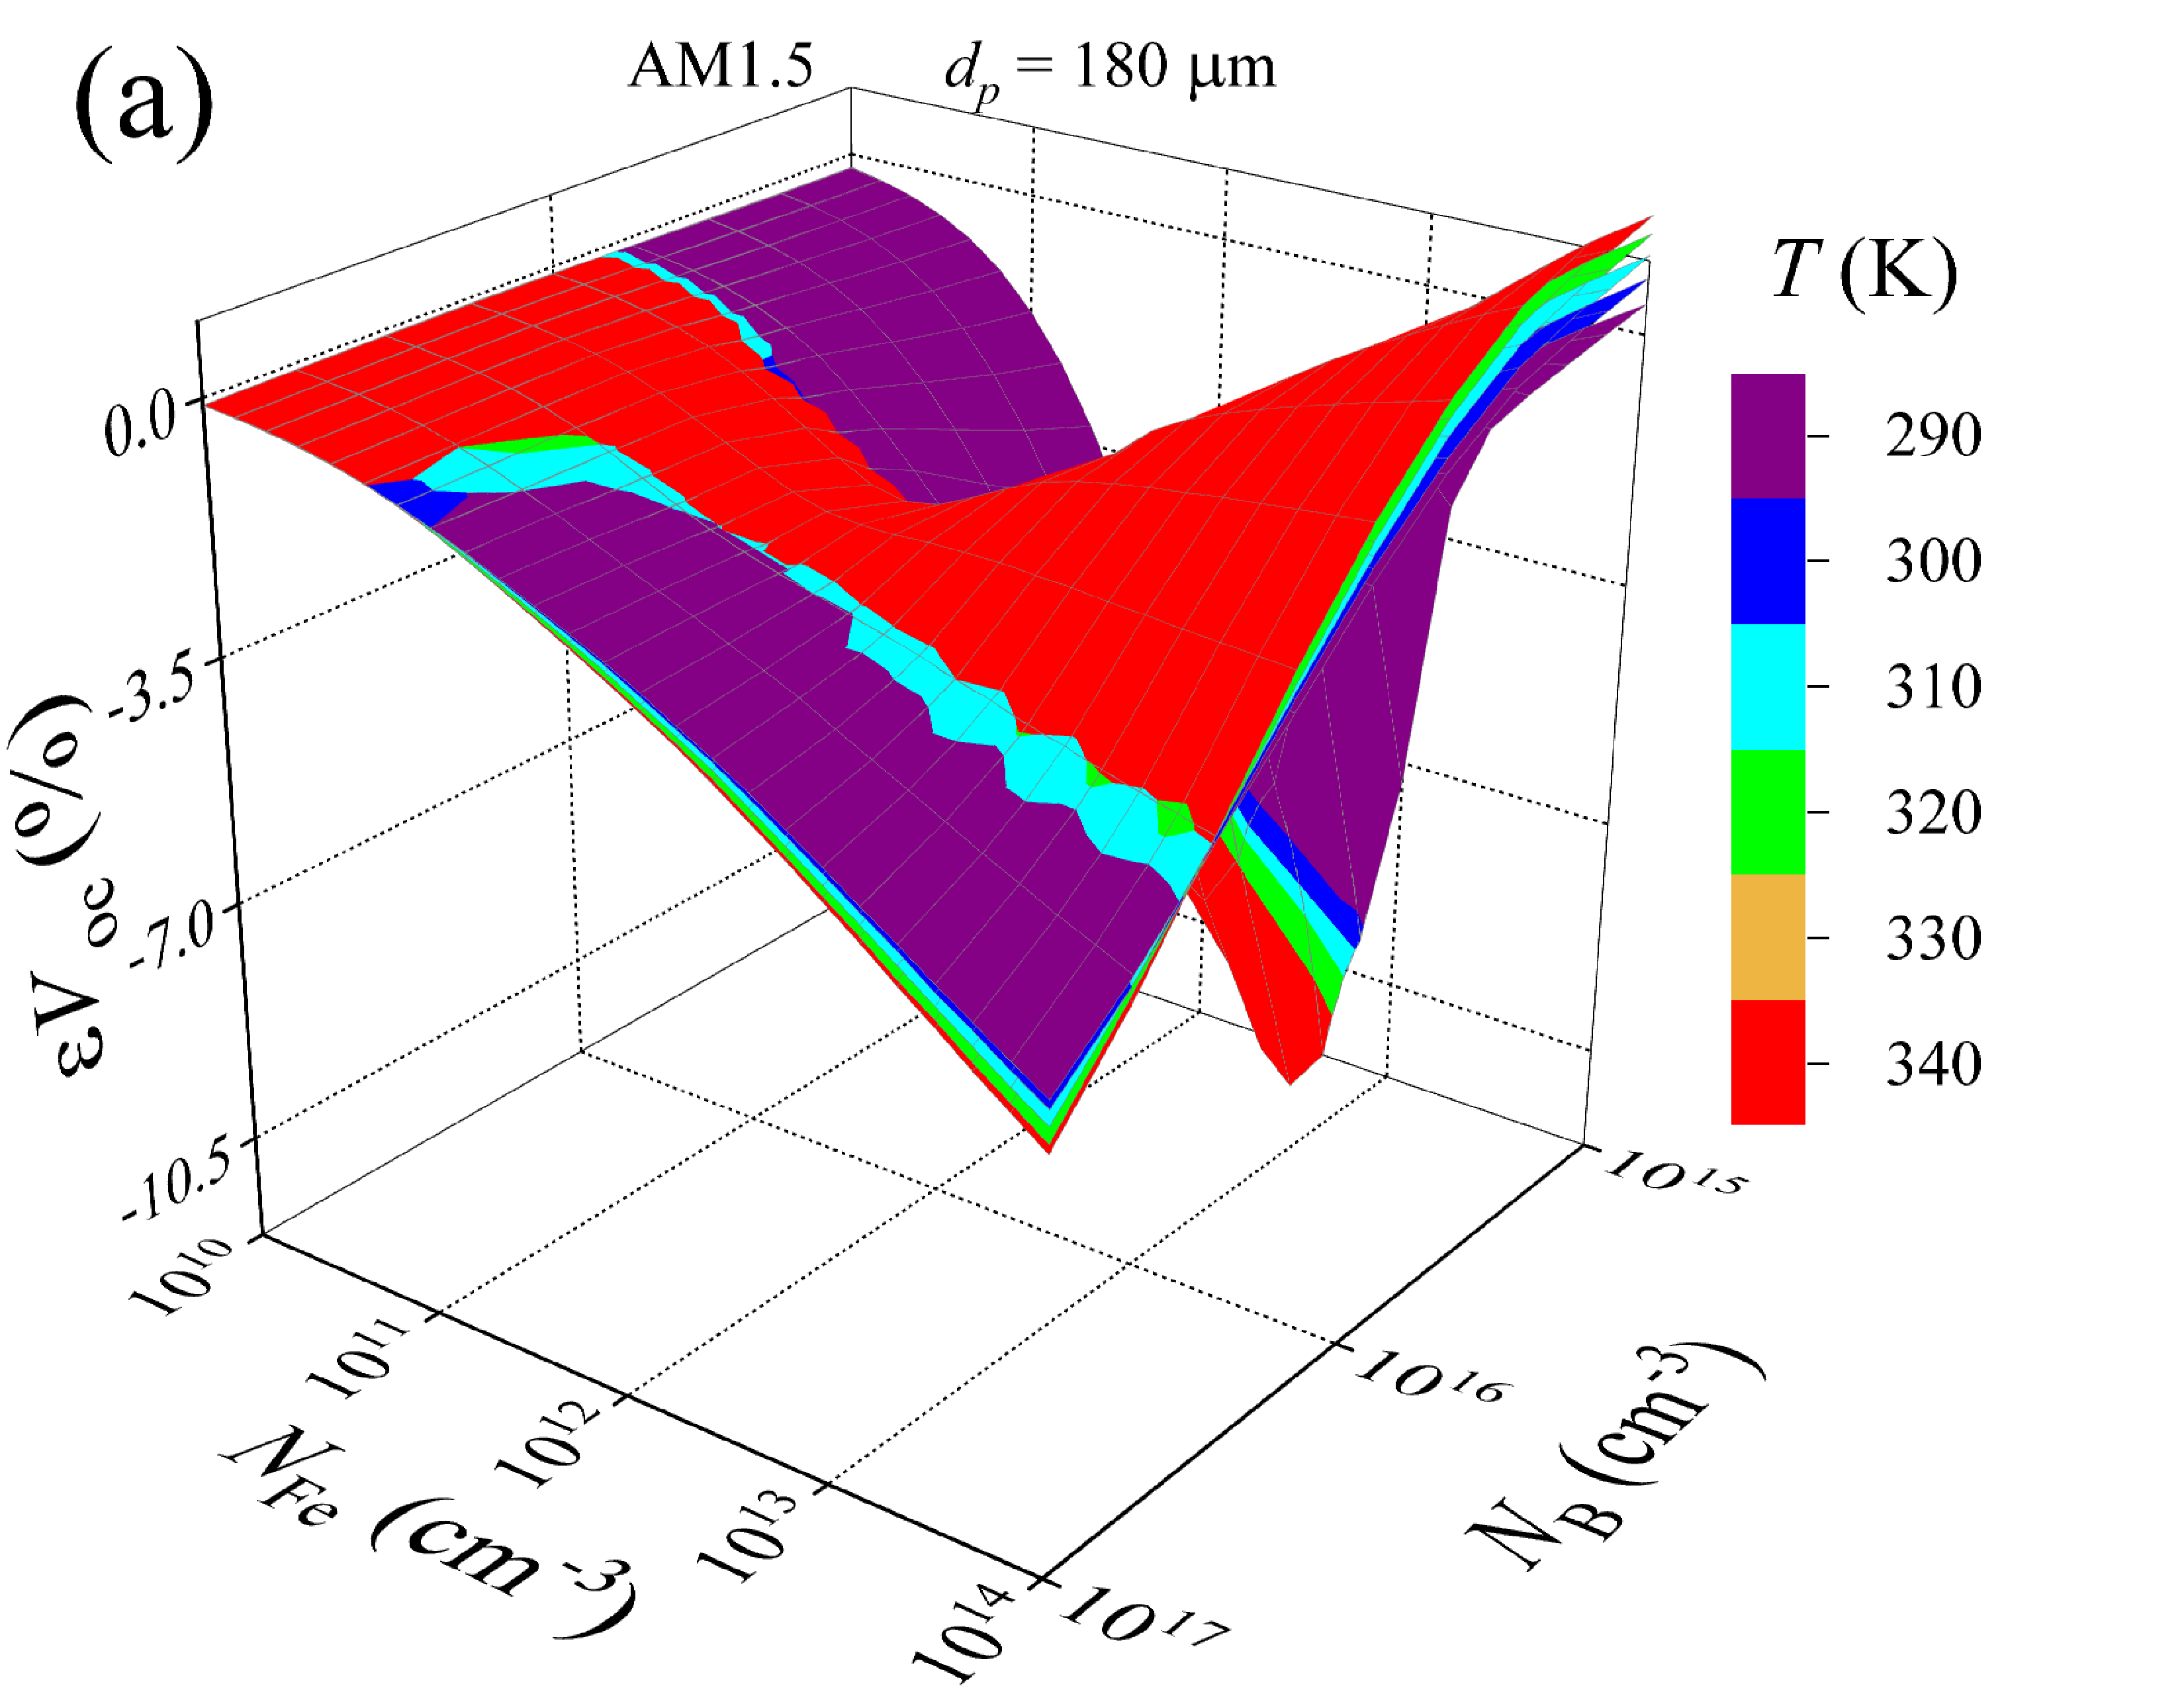
\includegraphics[width=0.49\linewidth]{Fig6a.png}
     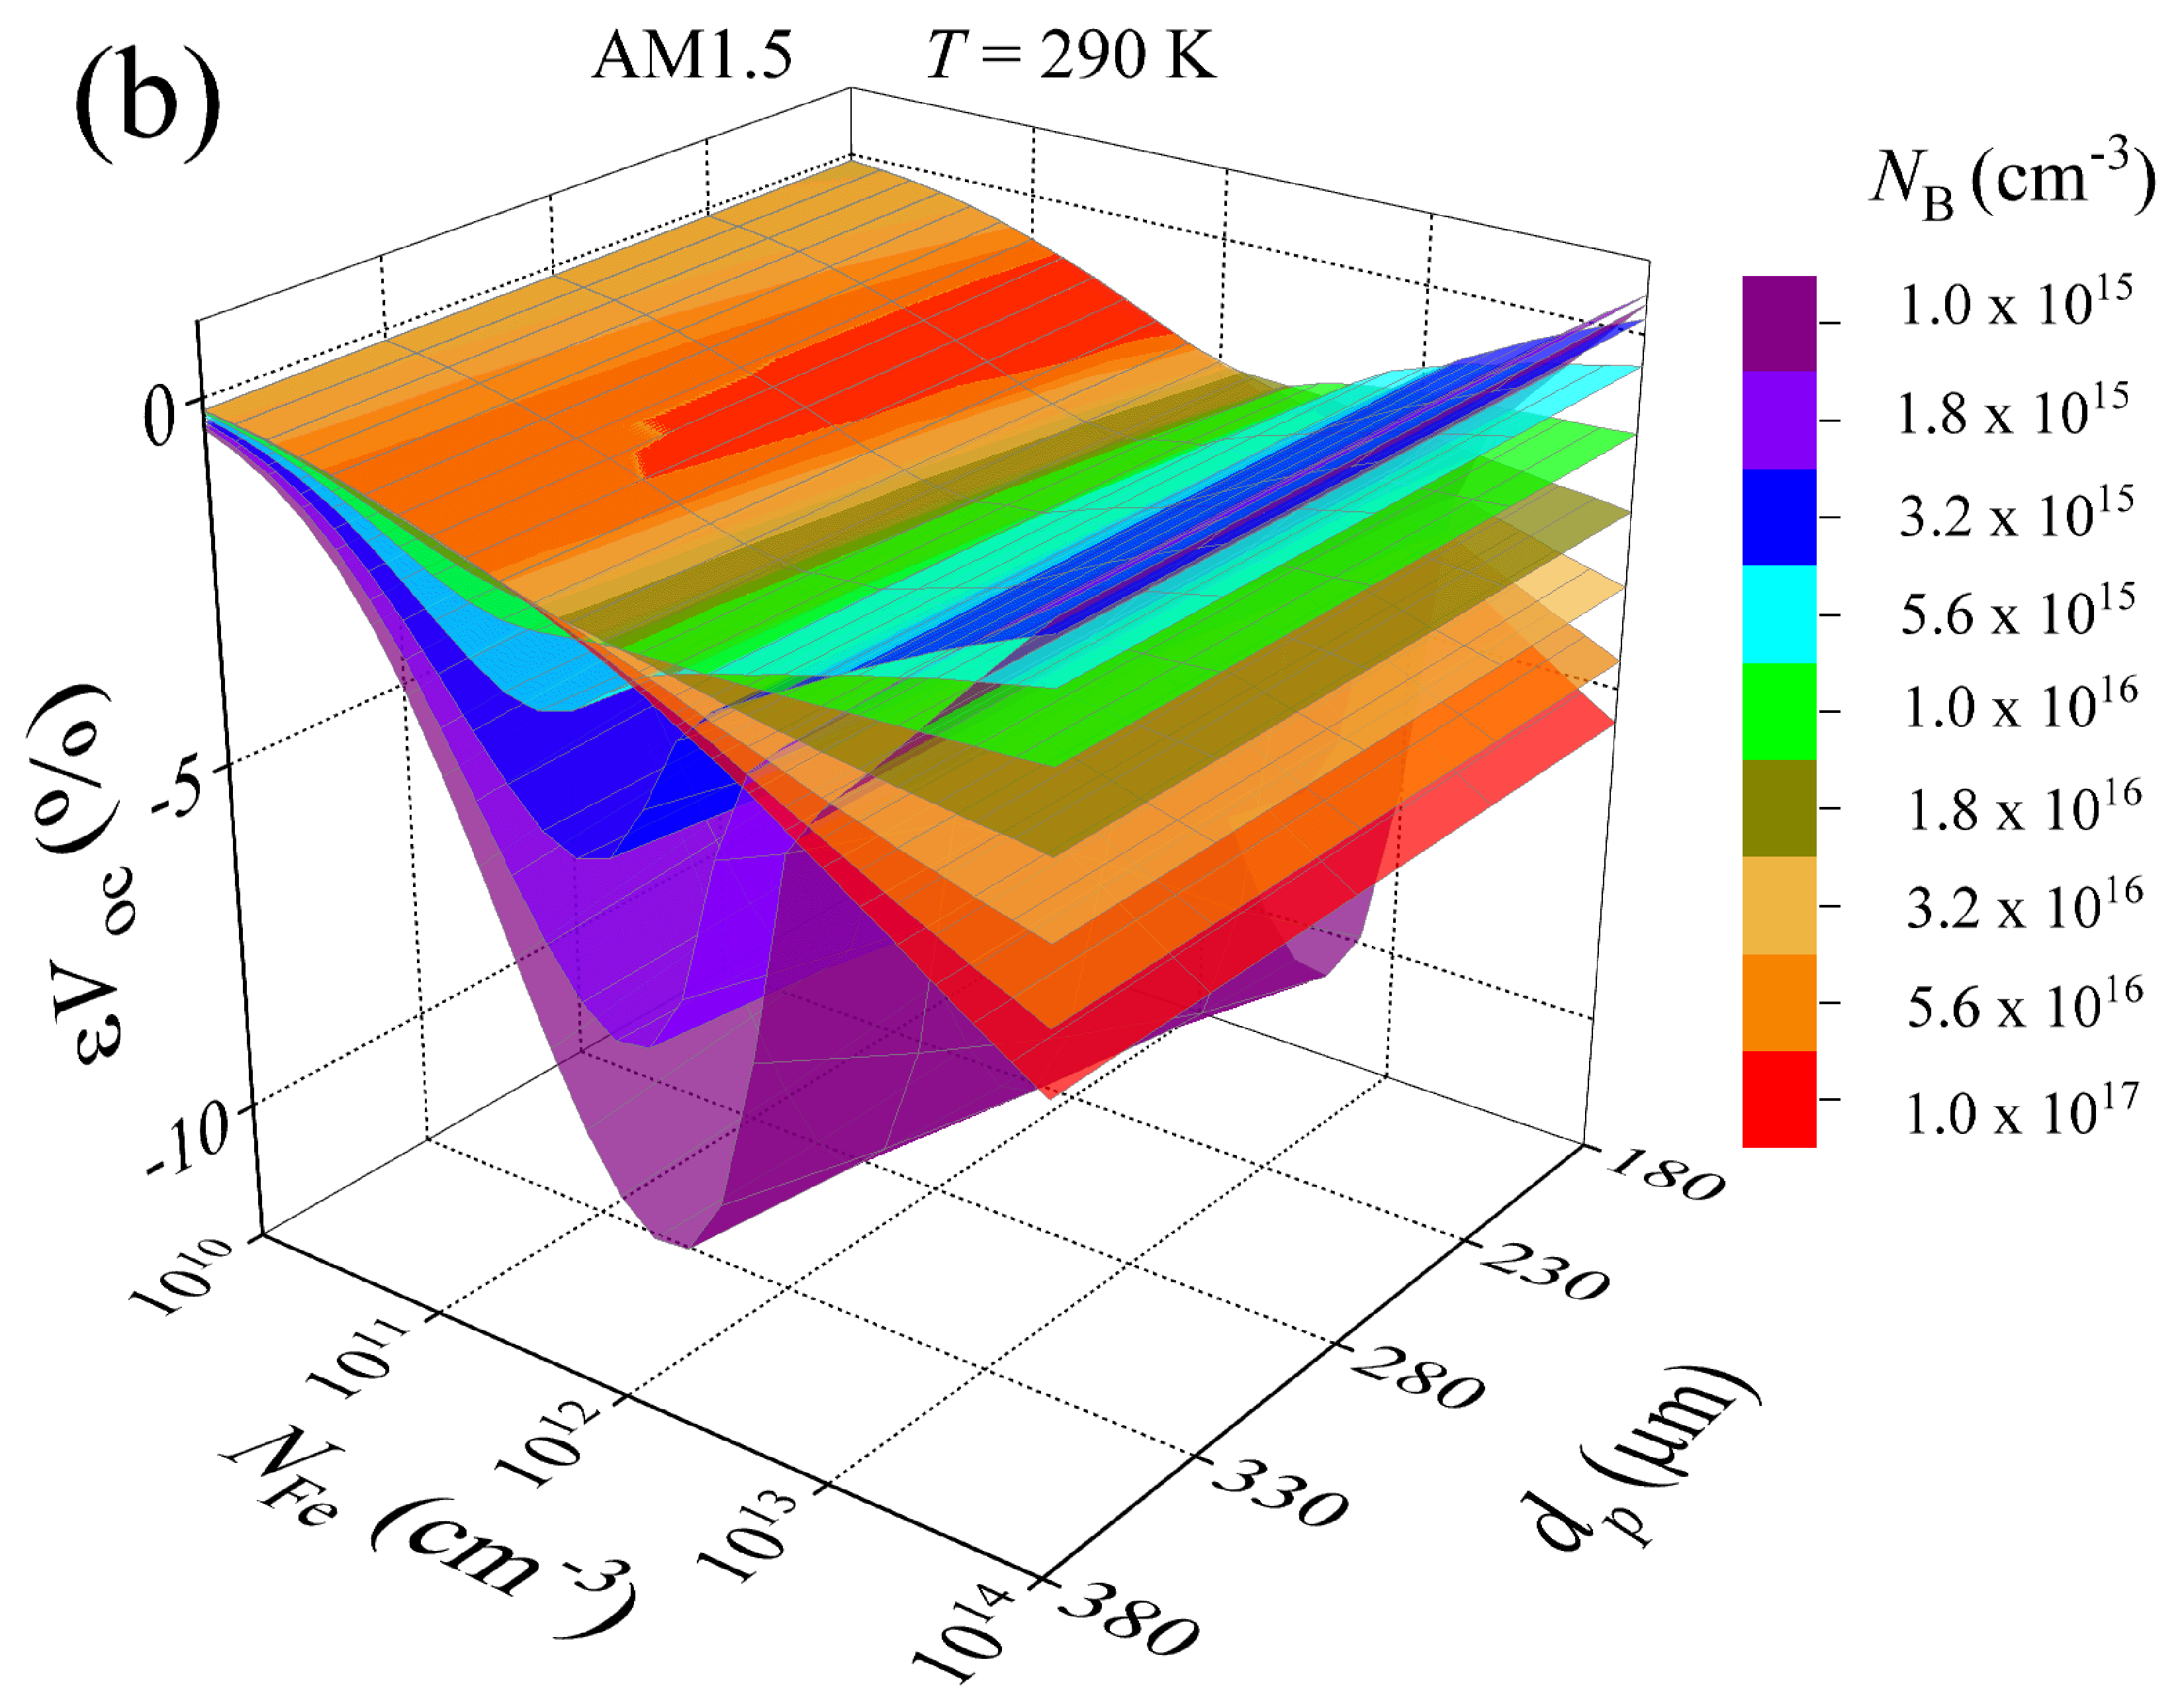
\includegraphics[width=0.49\linewidth]{Fig6b.png}
     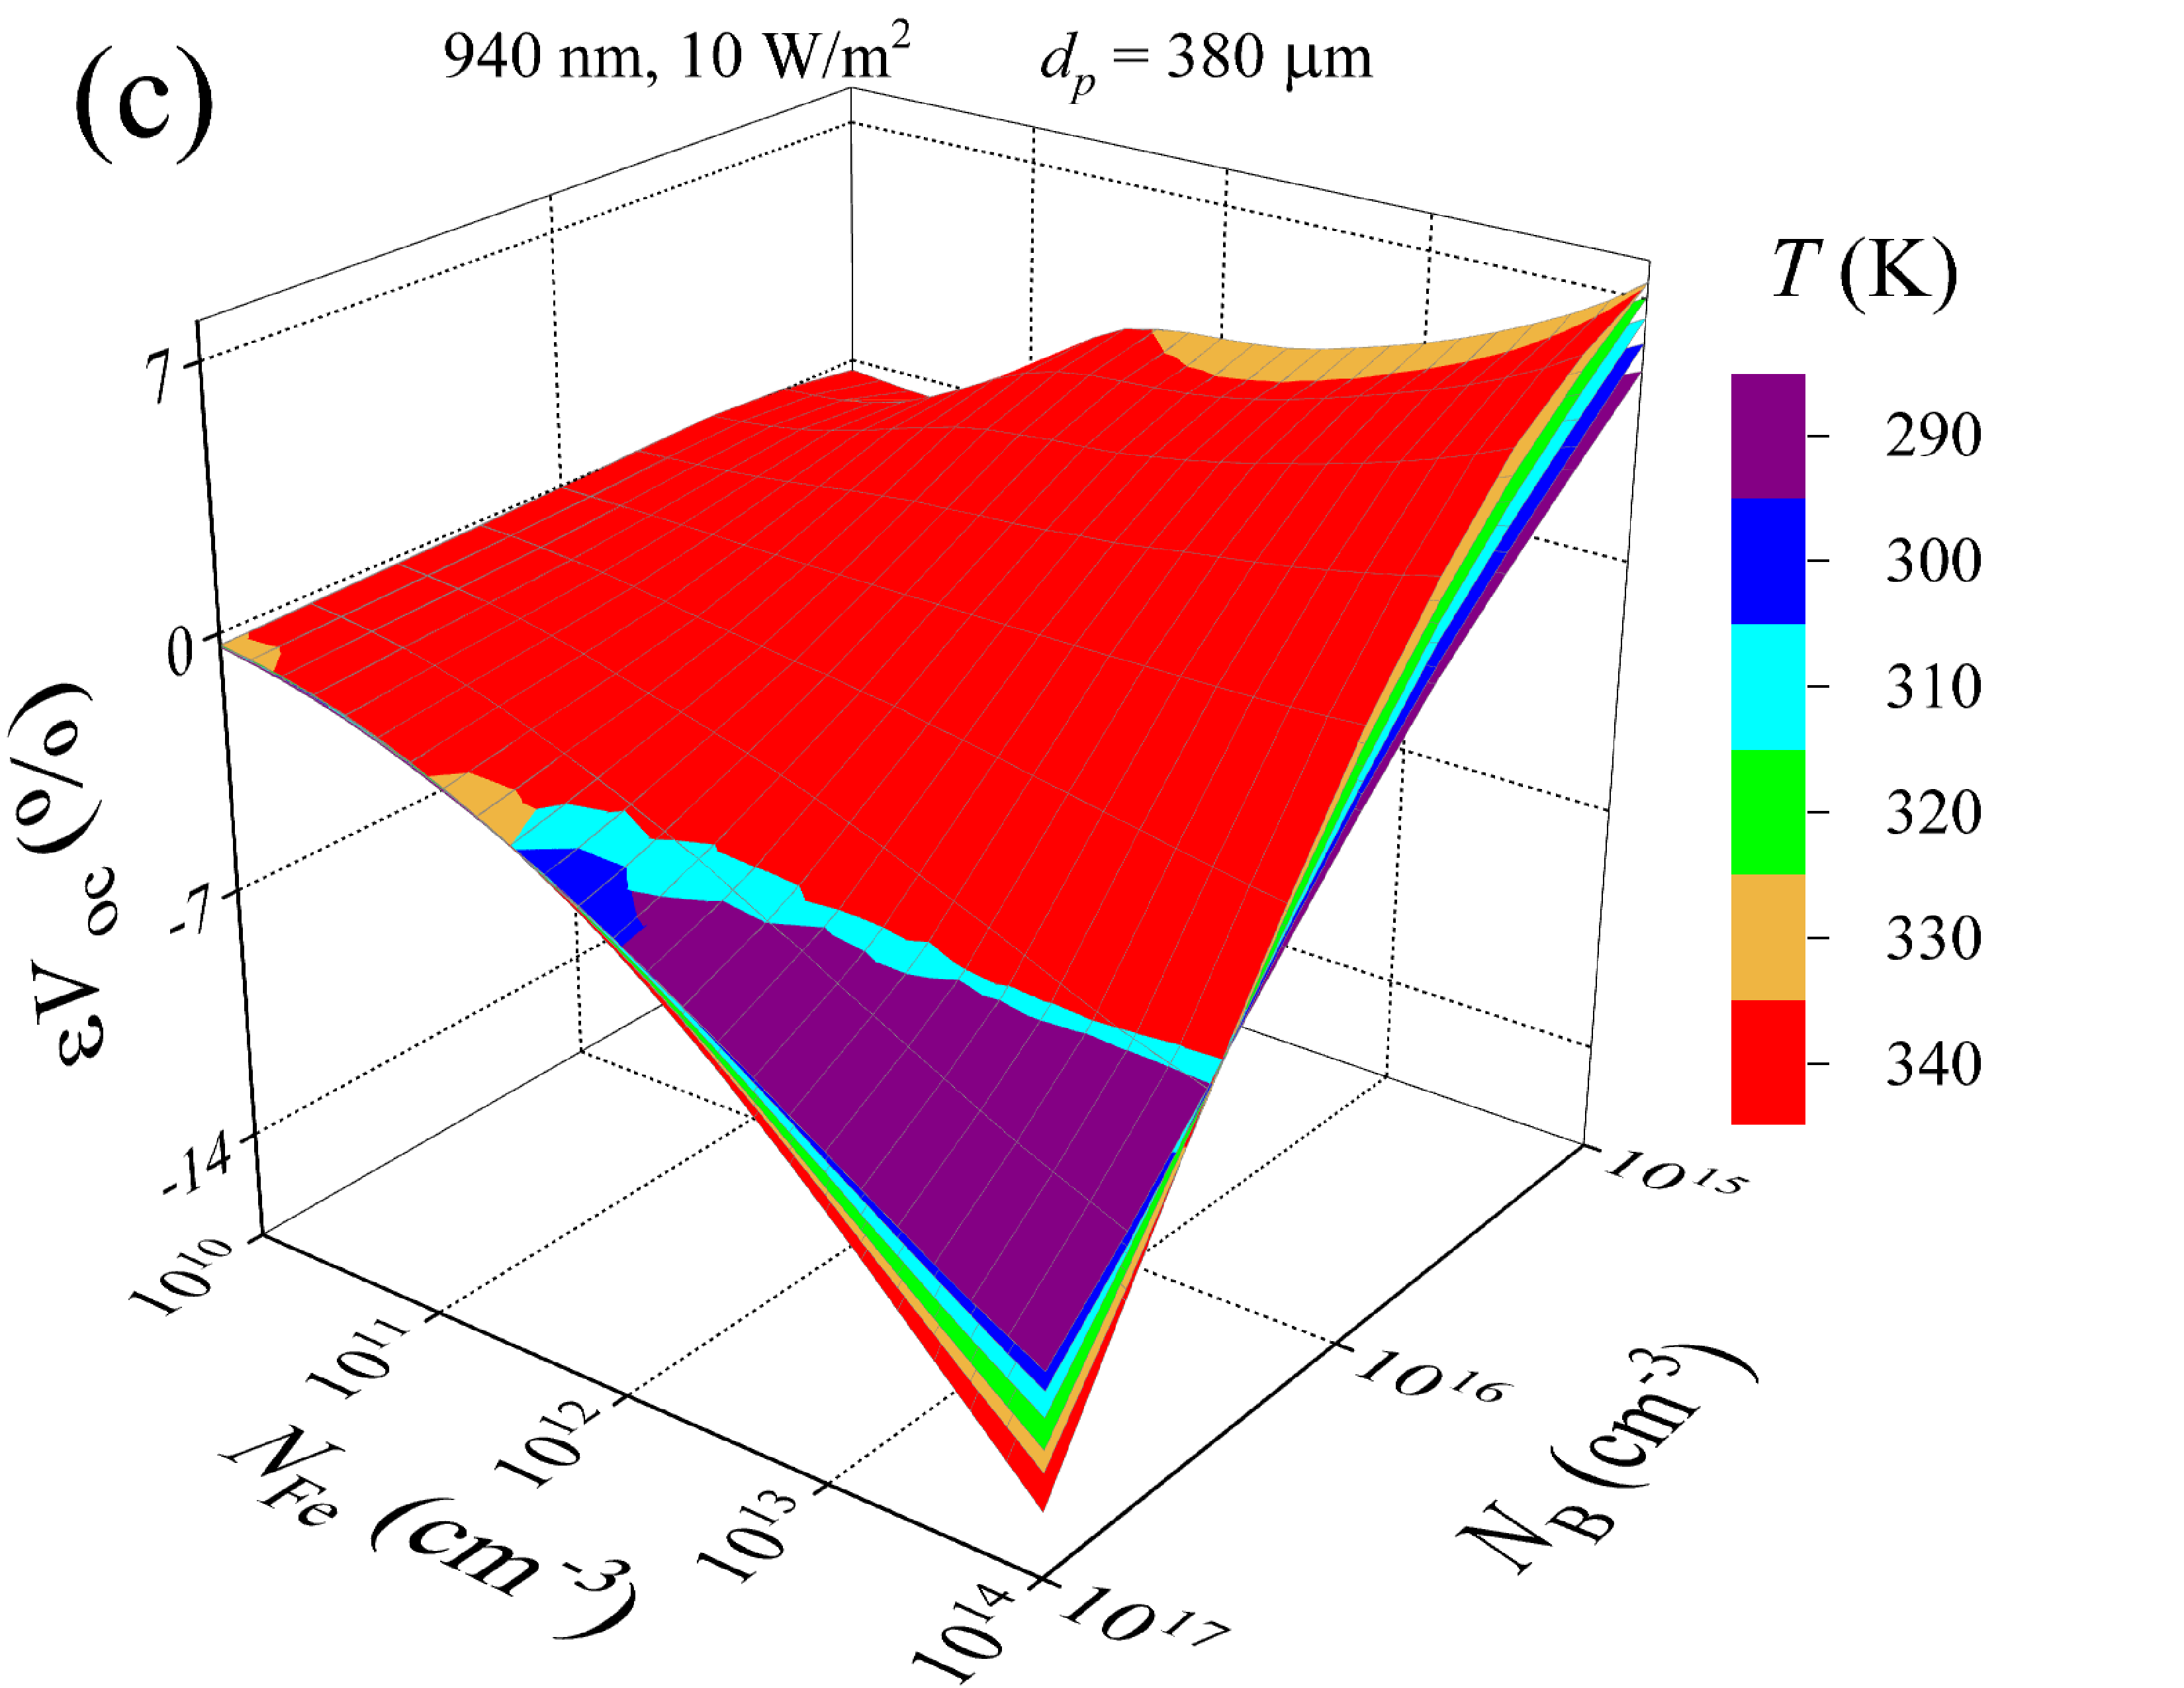
\includegraphics[width=0.49\linewidth]{Fig6c.png}
     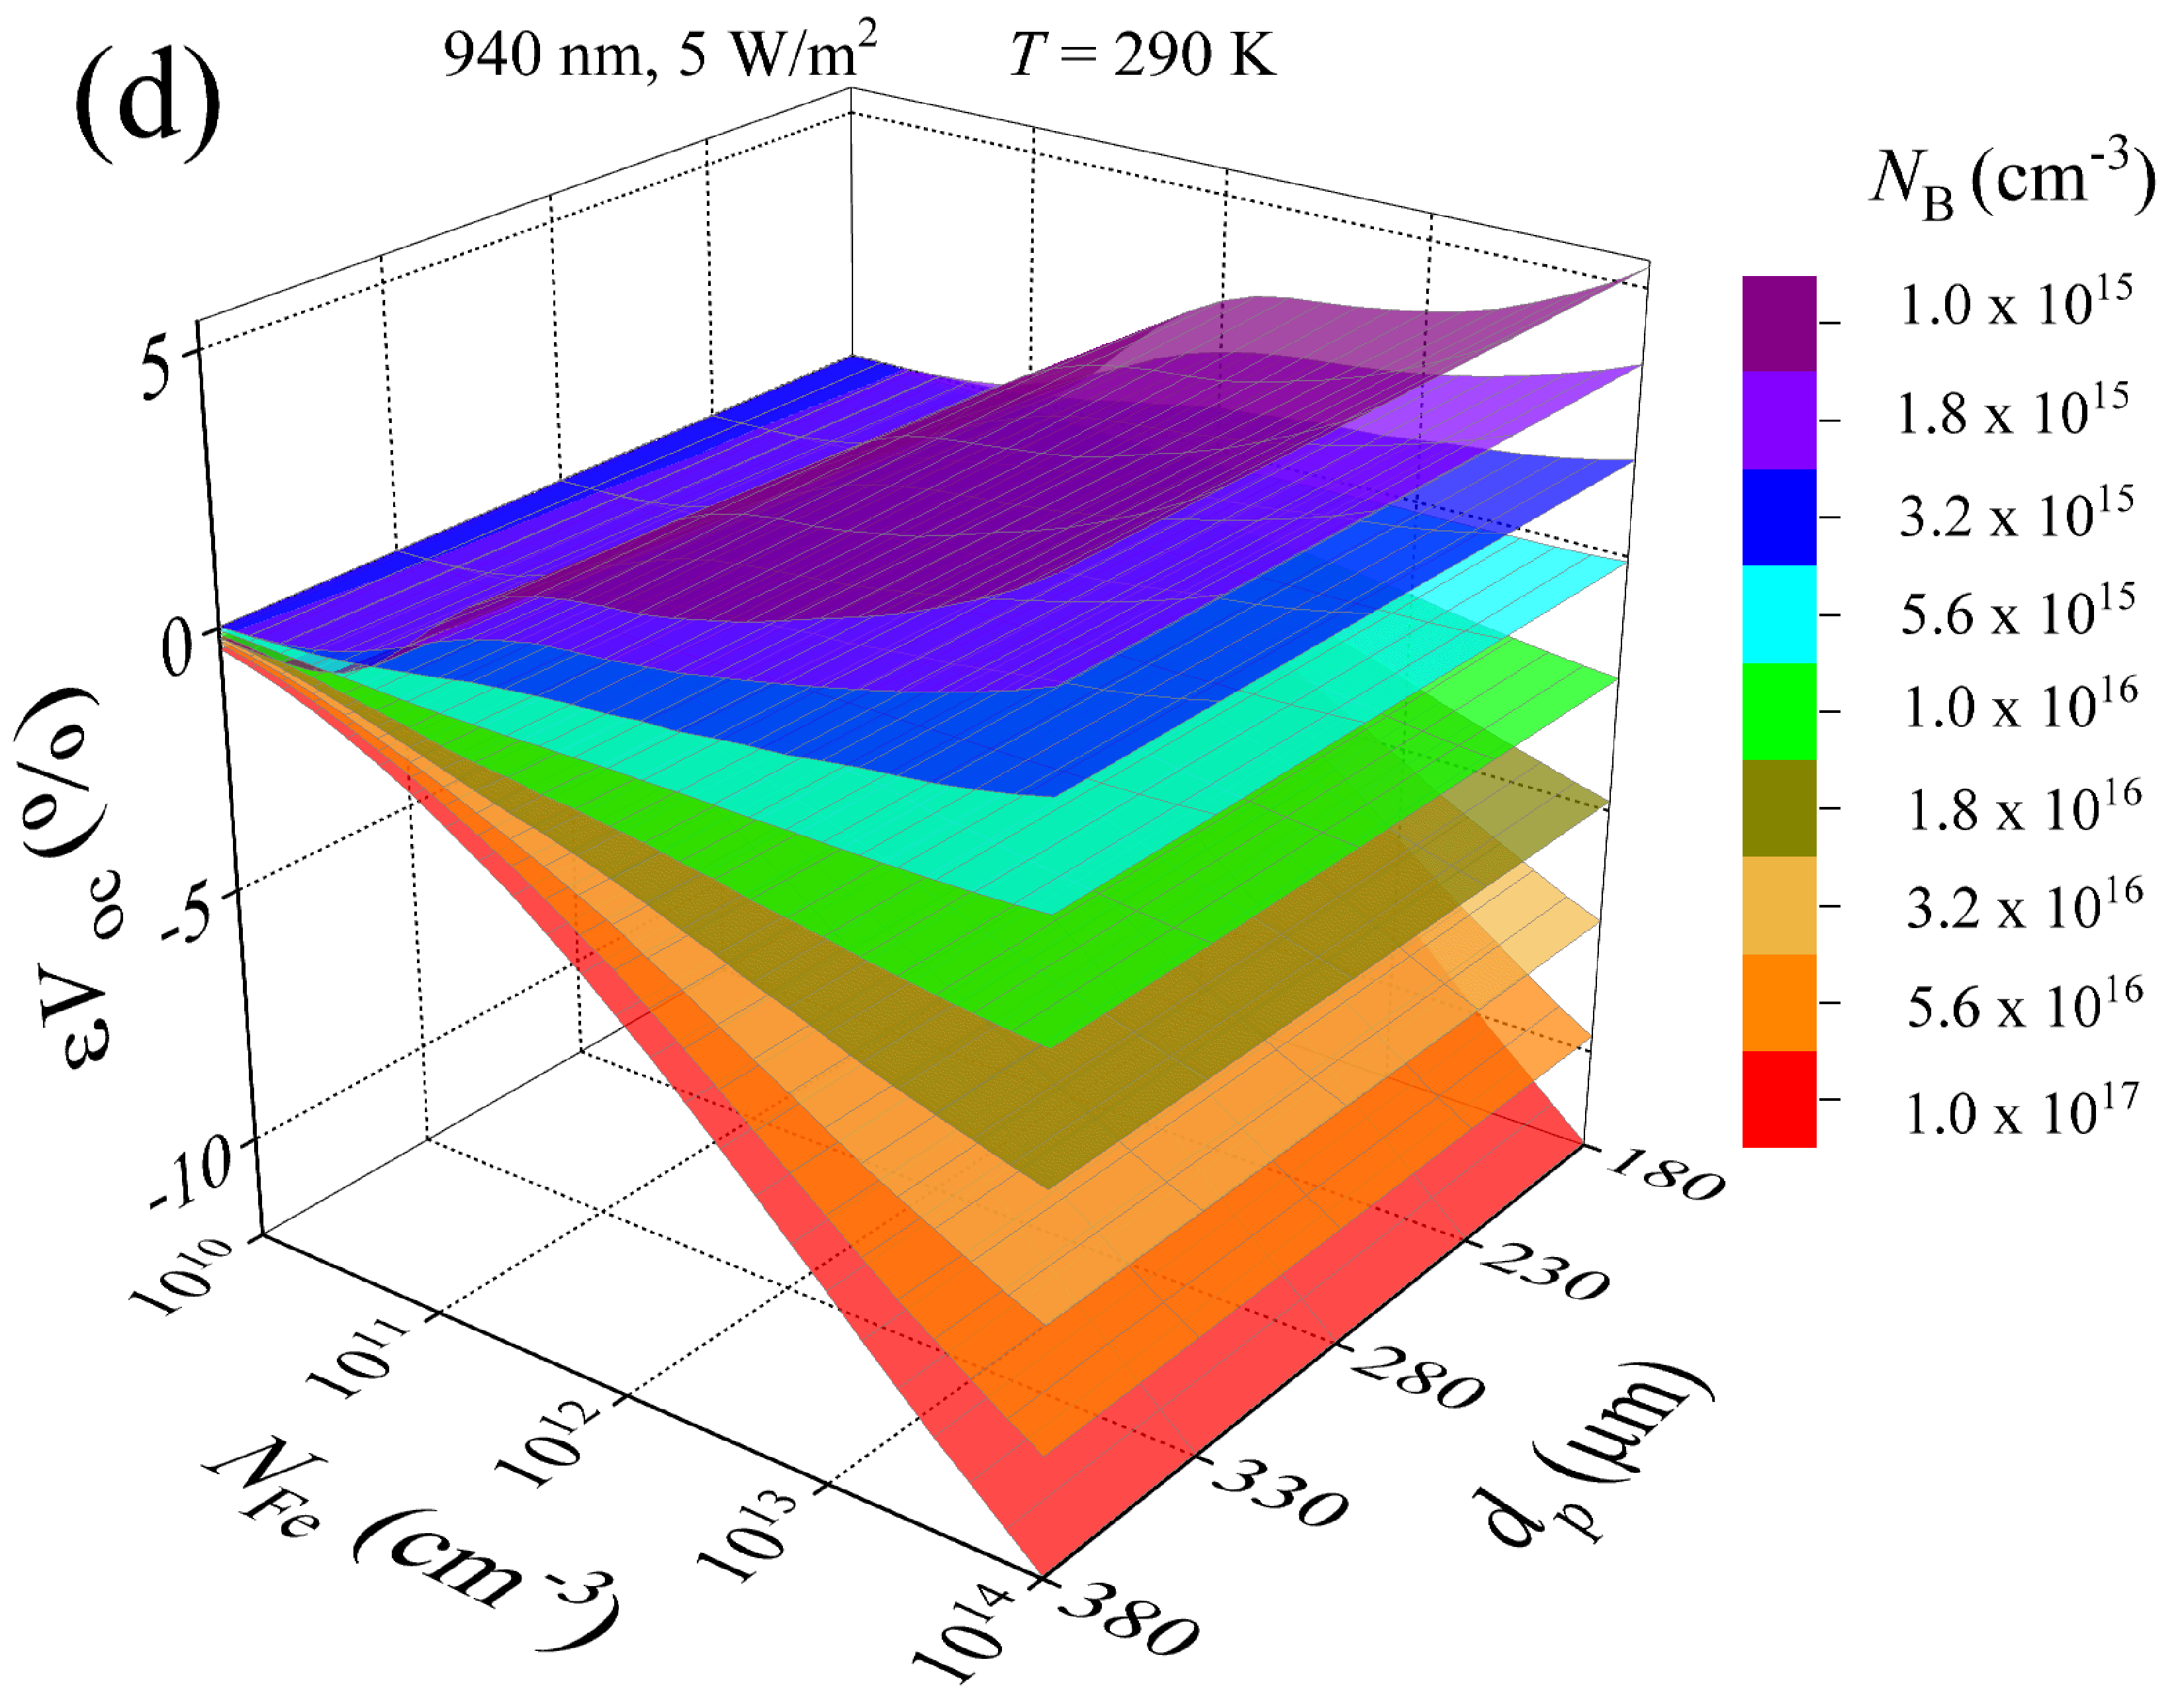
\includegraphics[width=0.49\linewidth]{Fig6d.png}
	  \caption{Dependencies of relative changes of open-circuit voltage on iron concentration and
       doping level (panels a and c) or base depth (b, d).
       Illumination: AM1.5 (a, b), 940~nm 10~Wm$^{-2}$ (c),  940~nm 5~Wm$^{-2}$ (d).
       $T$, K: 290 (b, d).
       Different surfaces correspond to different temperatures (a, c) and doping level (b, d).
}\label{fig6}
\end{figure}

\begin{figure}
	\centering
     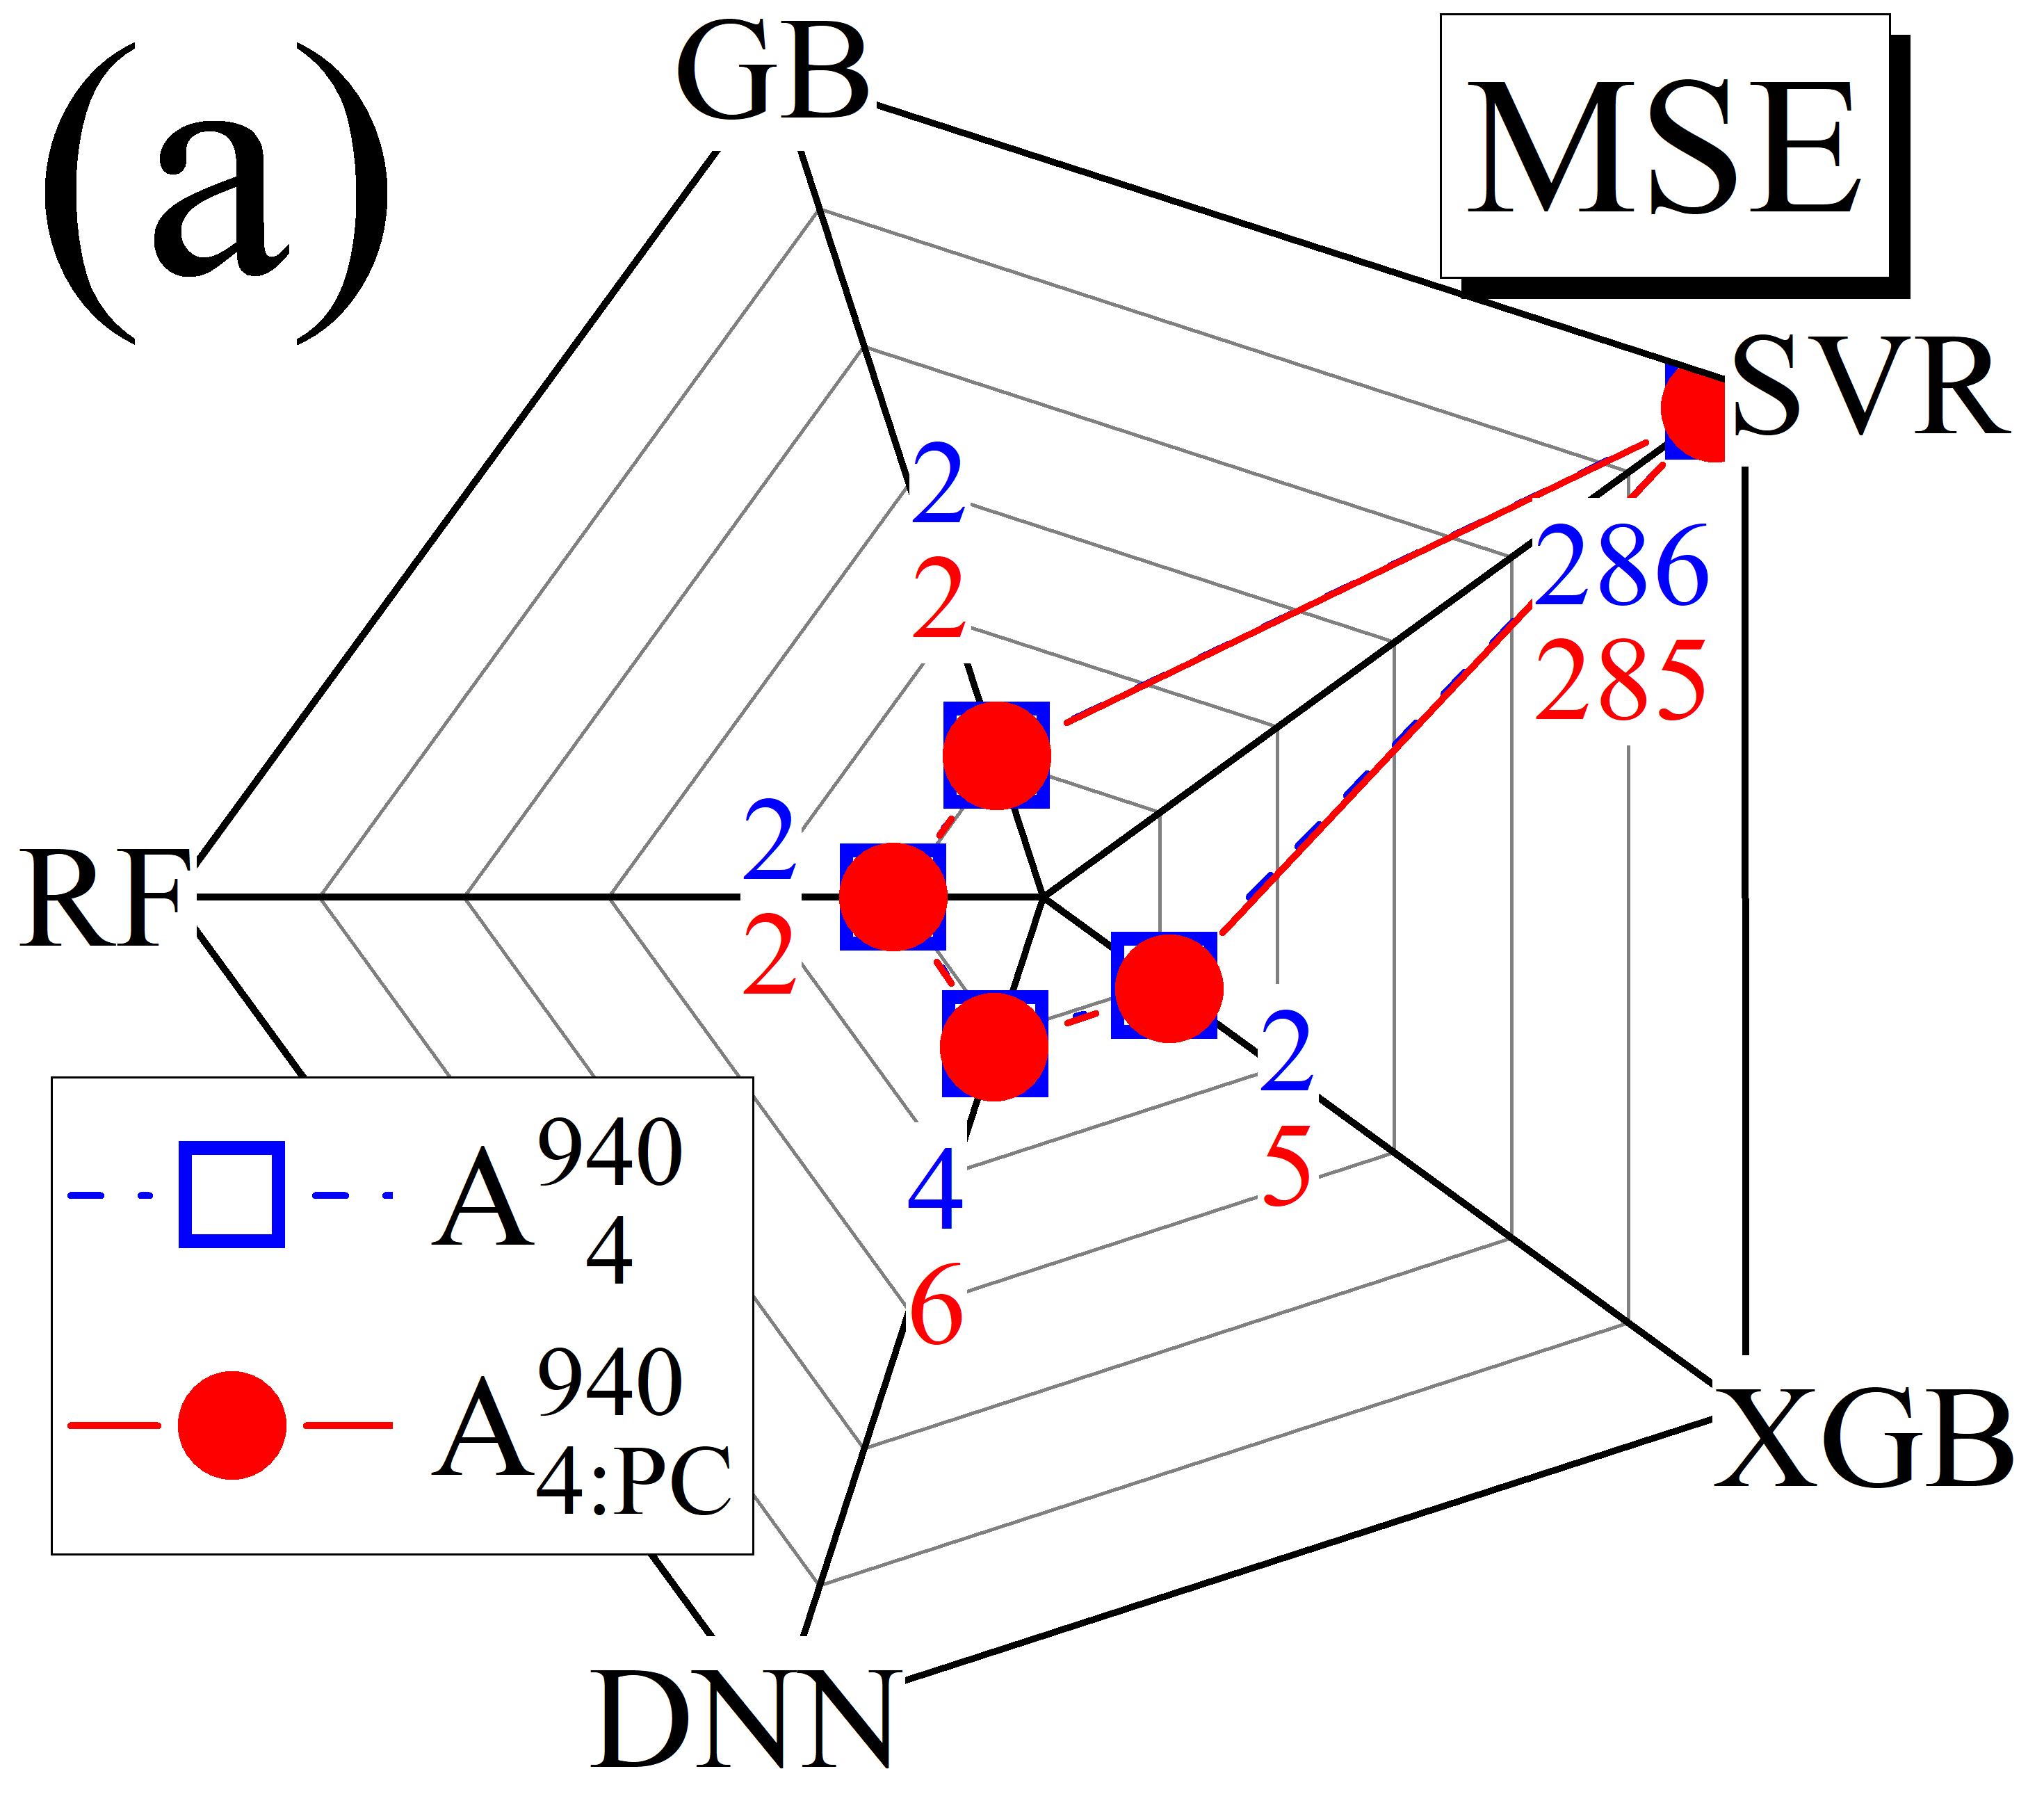
\includegraphics[width=0.4\linewidth]{Fig7a.png}
     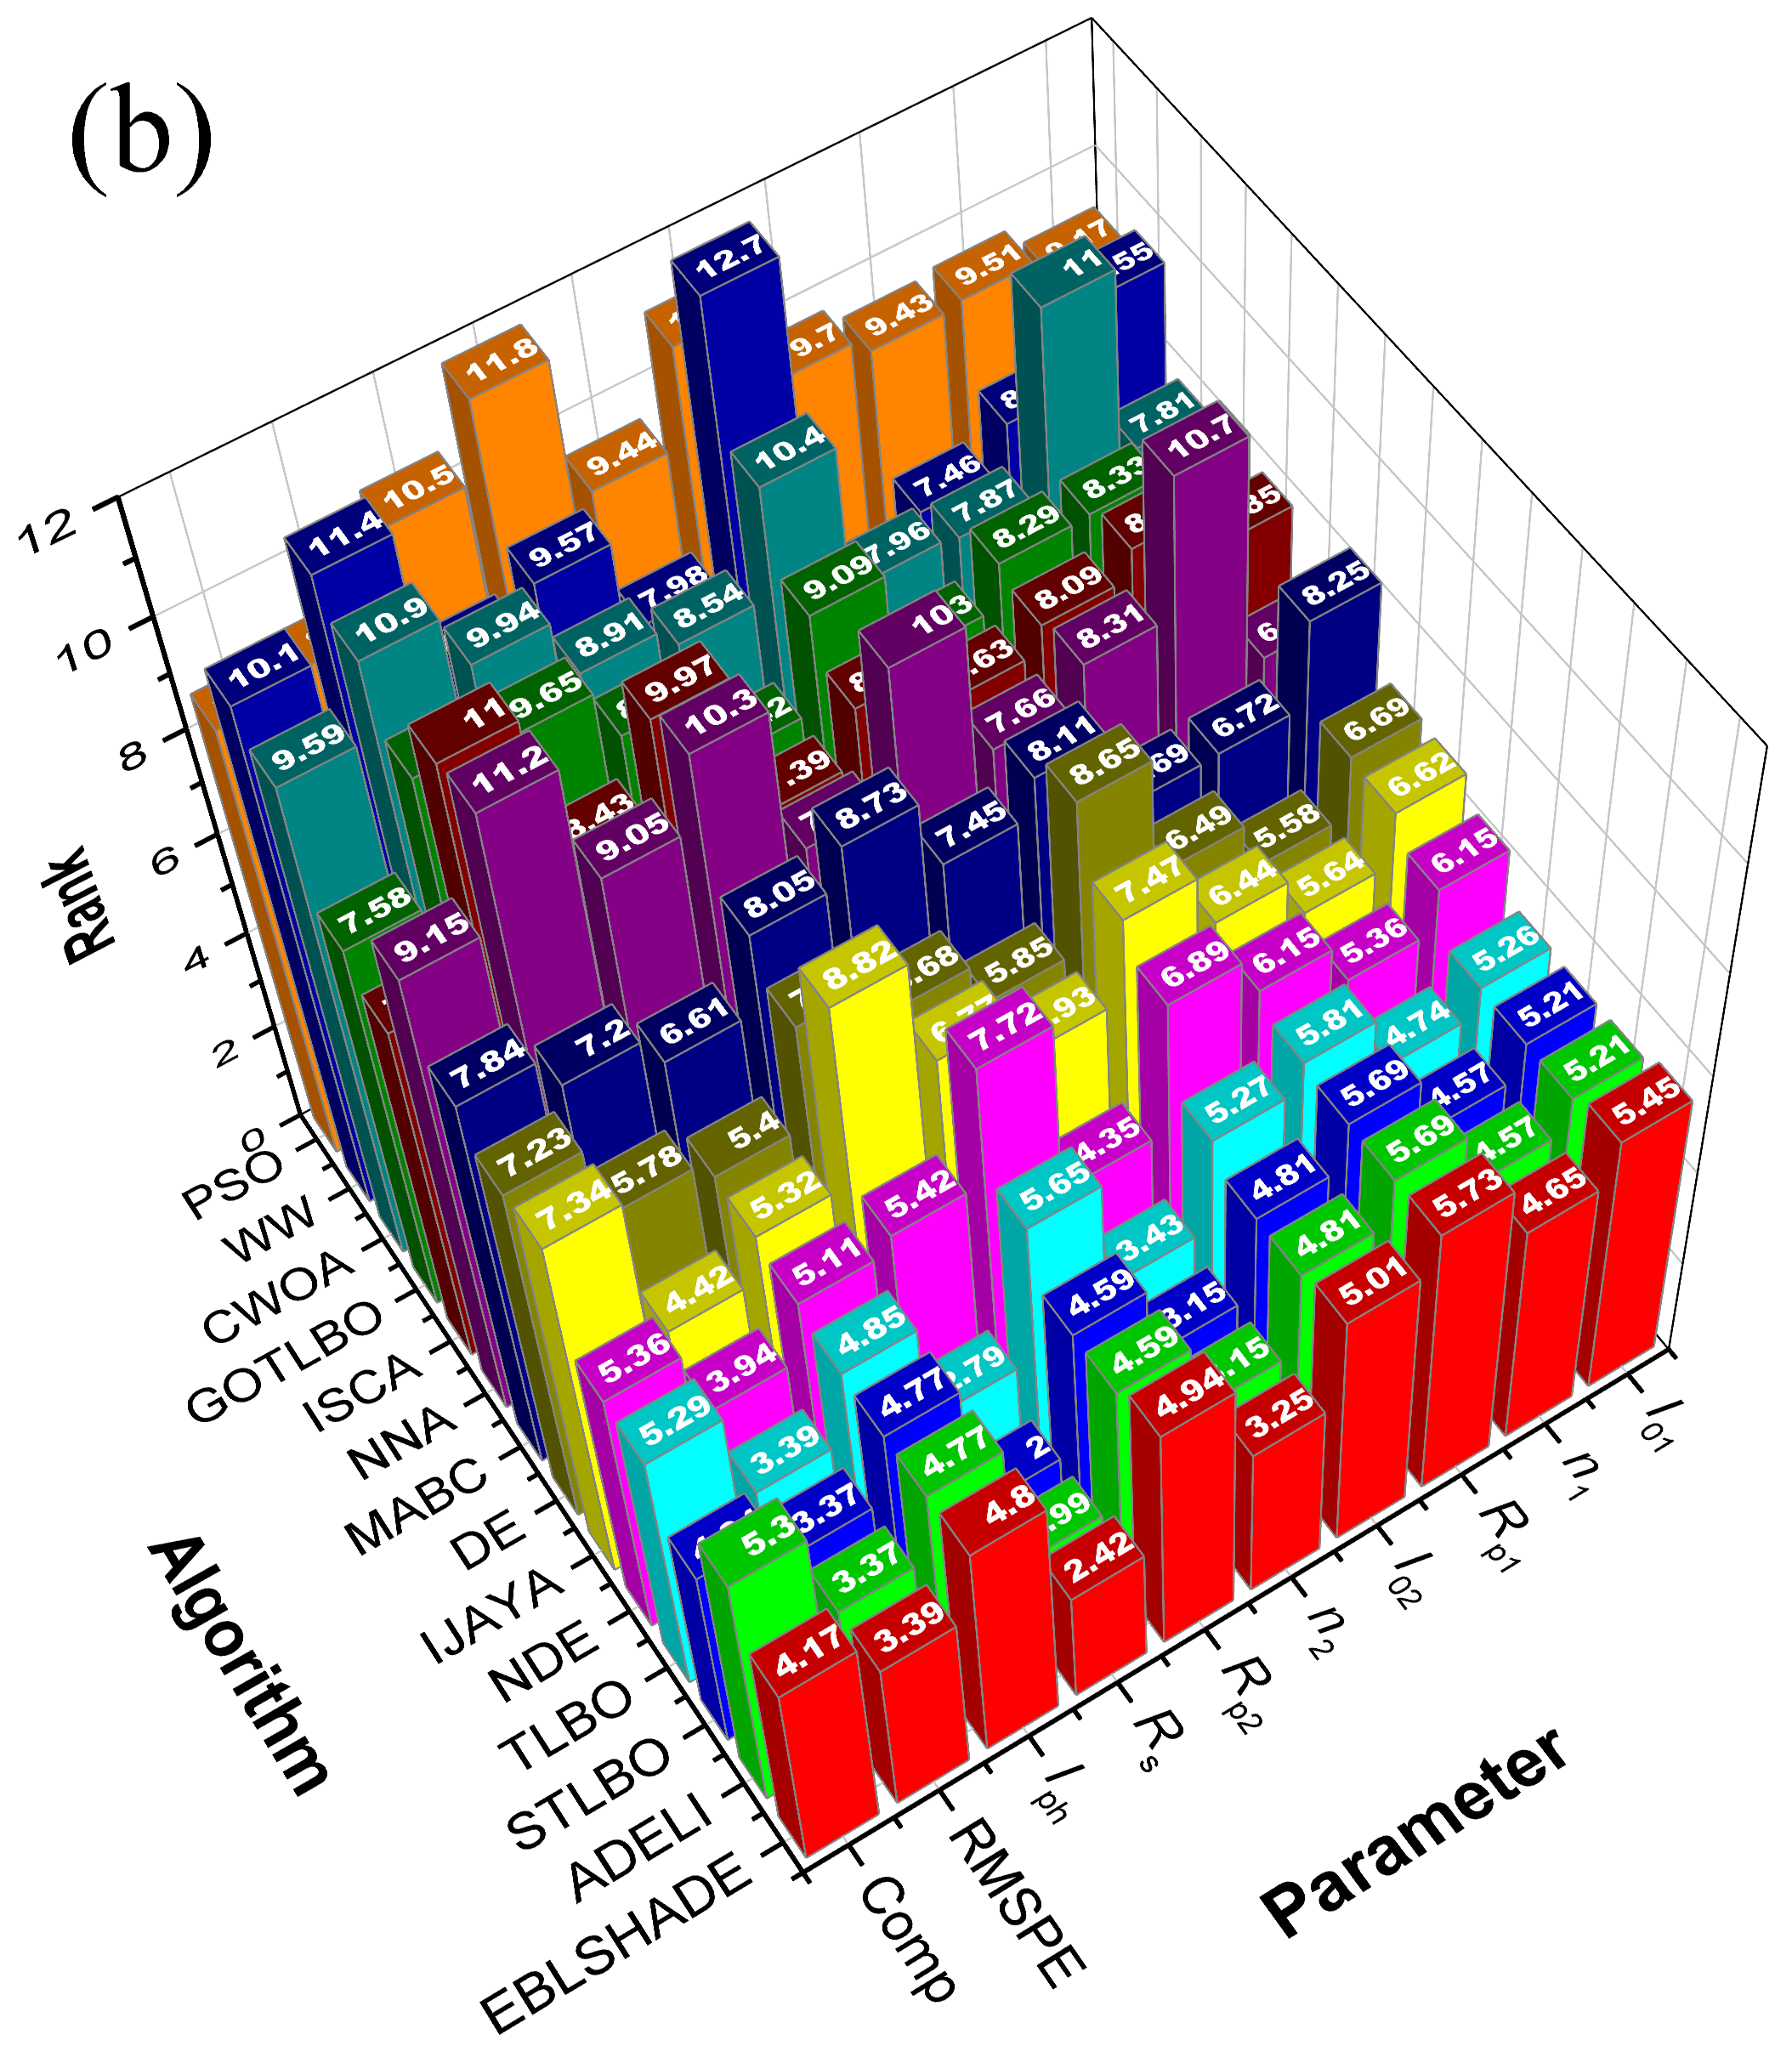
\includegraphics[width=0.4\linewidth]{Fig7b.png}
	  \caption{Dependencies of relative changes of open-circuit voltage on iron concentration (a) and
       temperature (b) for SSC with $d_p=380$~$\mu$m and $N_\mathrm{B}=1.36\times10^{15}$~cm$^{-3}$
       in the case of monochromatic (940~nm) illumination.
       The marks are the experimental results, the lines are the simulation results.
       $W_\mathrm{ill}$, Wm$^{-2}$: 5 (marks and solid lines), 10 (dotted lines).
       Different lines and marks correspond to different temperatures (a) or $N_\mathrm{Fe}$ values (b) --- see legends.
}\label{fig7}
\end{figure}

\subsection{Fill factor}

\subsection{Solar Cell Efficiency}



\section{Conclusion}
%--------------------------------------------------------


% Numbered list
% Use the style of numbering in square brackets.
% If nothing is used, default style will be taken.
%\begin{enumerate}[a)]
%\item
%\item
%\item
%\end{enumerate}

% Unnumbered list
%\begin{itemize}
%\item
%\item
%\item
%\end{itemize}

% Description list
%\begin{description}
%\item[]
%\item[]
%\item[]
%\end{description}

% Figure
%\begin{figure}[<options>]
%	\centering
%		\includegraphics[<options>]{}
%	  \caption{}\label{fig1}
%\end{figure}


%\begin{table}[<options>]
%\caption{}\label{tbl1}
%\begin{tabular*}{\tblwidth}{@{}LL@{}}
%\toprule
%  &  \\ % Table header row
%\midrule
% & \\
% & \\
% & \\
% & \\
%\bottomrule
%\end{tabular*}
%\end{table}

% Uncomment and use as the case may be
%\begin{theorem}
%\end{theorem}

% Uncomment and use as the case may be
%\begin{lemma}
%\end{lemma}

%% The Appendices part is started with the command \appendix;
%% appendix sections are then done as normal sections
%% \appendix

%\section{}\label{}

% To print the credit authorship contribution details
\printcredits

%% Loading bibliography style file
\bibliographystyle{model1-num-names}

%\bibliographystyle{cas-model2-names}

% Loading bibliography database
\bibliography{olikh}

% Biography
%\bio{}
%% Here goes the biography details.
%\endbio
%
%\bio{pic1}
%% Here goes the biography details.
%\endbio

\end{document}

